\documentclass[10pt, xcolor=x11names,compress]{beamer}
\usepackage{tabulary}
\usepackage{booktabs}
\usepackage{float}
\usepackage{graphicx}
\usepackage{mwe}% for example pictures
\usepackage{siunitx}
\usepackage{hyperref}

\definecolor{sangria}{rgb}{0.57, 0.0, 0.04}
\usecolortheme[named=sangria]{structure}
\useoutertheme{infolines}
\usefonttheme[onlymath]{serif}
\setbeamertemplate{headline}[default]
\setbeamertemplate{navigation symbols}{}
\mode<beamer>{\setbeamertemplate{blocks}[rounded][shadow=true]}
\setbeamercovered{transparent}
\setbeamercolor{block body}{use=structure, fg=white, bg=black!20}
\setbeamercolor{itemize item}{fg=black}
\setbeamercolor{itemize subitem}{fg=gray} 
\setbeamercolor{itemize subsubitem}{fg=black!20} 
\makeatletter\setbeamertemplate{footline}
{  
	\leavevmode%  
	\hbox{%  
		\begin{beamercolorbox}[wd=.333333\paperwidth,ht=2.25ex,dp=1ex,center]{author in head/foot}%    
			\usebeamerfont{author in head/foot}
			\insertshortauthor%~~\beamer@ifempty{\insertshortinstitute}{}
		\end{beamercolorbox}%  
		\begin{beamercolorbox}[wd=.333333\paperwidth,ht=2.25ex,dp=1ex,center]{institute in head/foot}%    
			\usebeamerfont{title in head/foot}\insertinstitute  
		\end{beamercolorbox}%  
		\begin{beamercolorbox}[wd=.333333\paperwidth,ht=2.25ex,dp=1ex,right]{date in head/foot}%    
			\usebeamerfont{date in head/foot}\insertshortdate{}\hspace*{2em}    
			\insertframenumber{} / \inserttotalframenumber\hspace*{2ex}   
	\end{beamercolorbox}}%  
	\vskip0pt%
}
\makeatother 
\useoutertheme[footline=empty, subsection=false]{miniframes}
\usepackage{multicol}  
\author{Núcleo de Estudos Raciais}
\title{Apresentação - Resultados Preliminares Carta de Conjuntura Mercado de Trabalho}

\institute{Insper}\date{10/07/2024} 
\begin{document}
	\begin{frame}
		\titlepage
	\end{frame}
	
	
	\section{Contexto} 
	\begin{frame}{Rendimento Recente do Trabalho}
		\begin{figure}
			\centering
			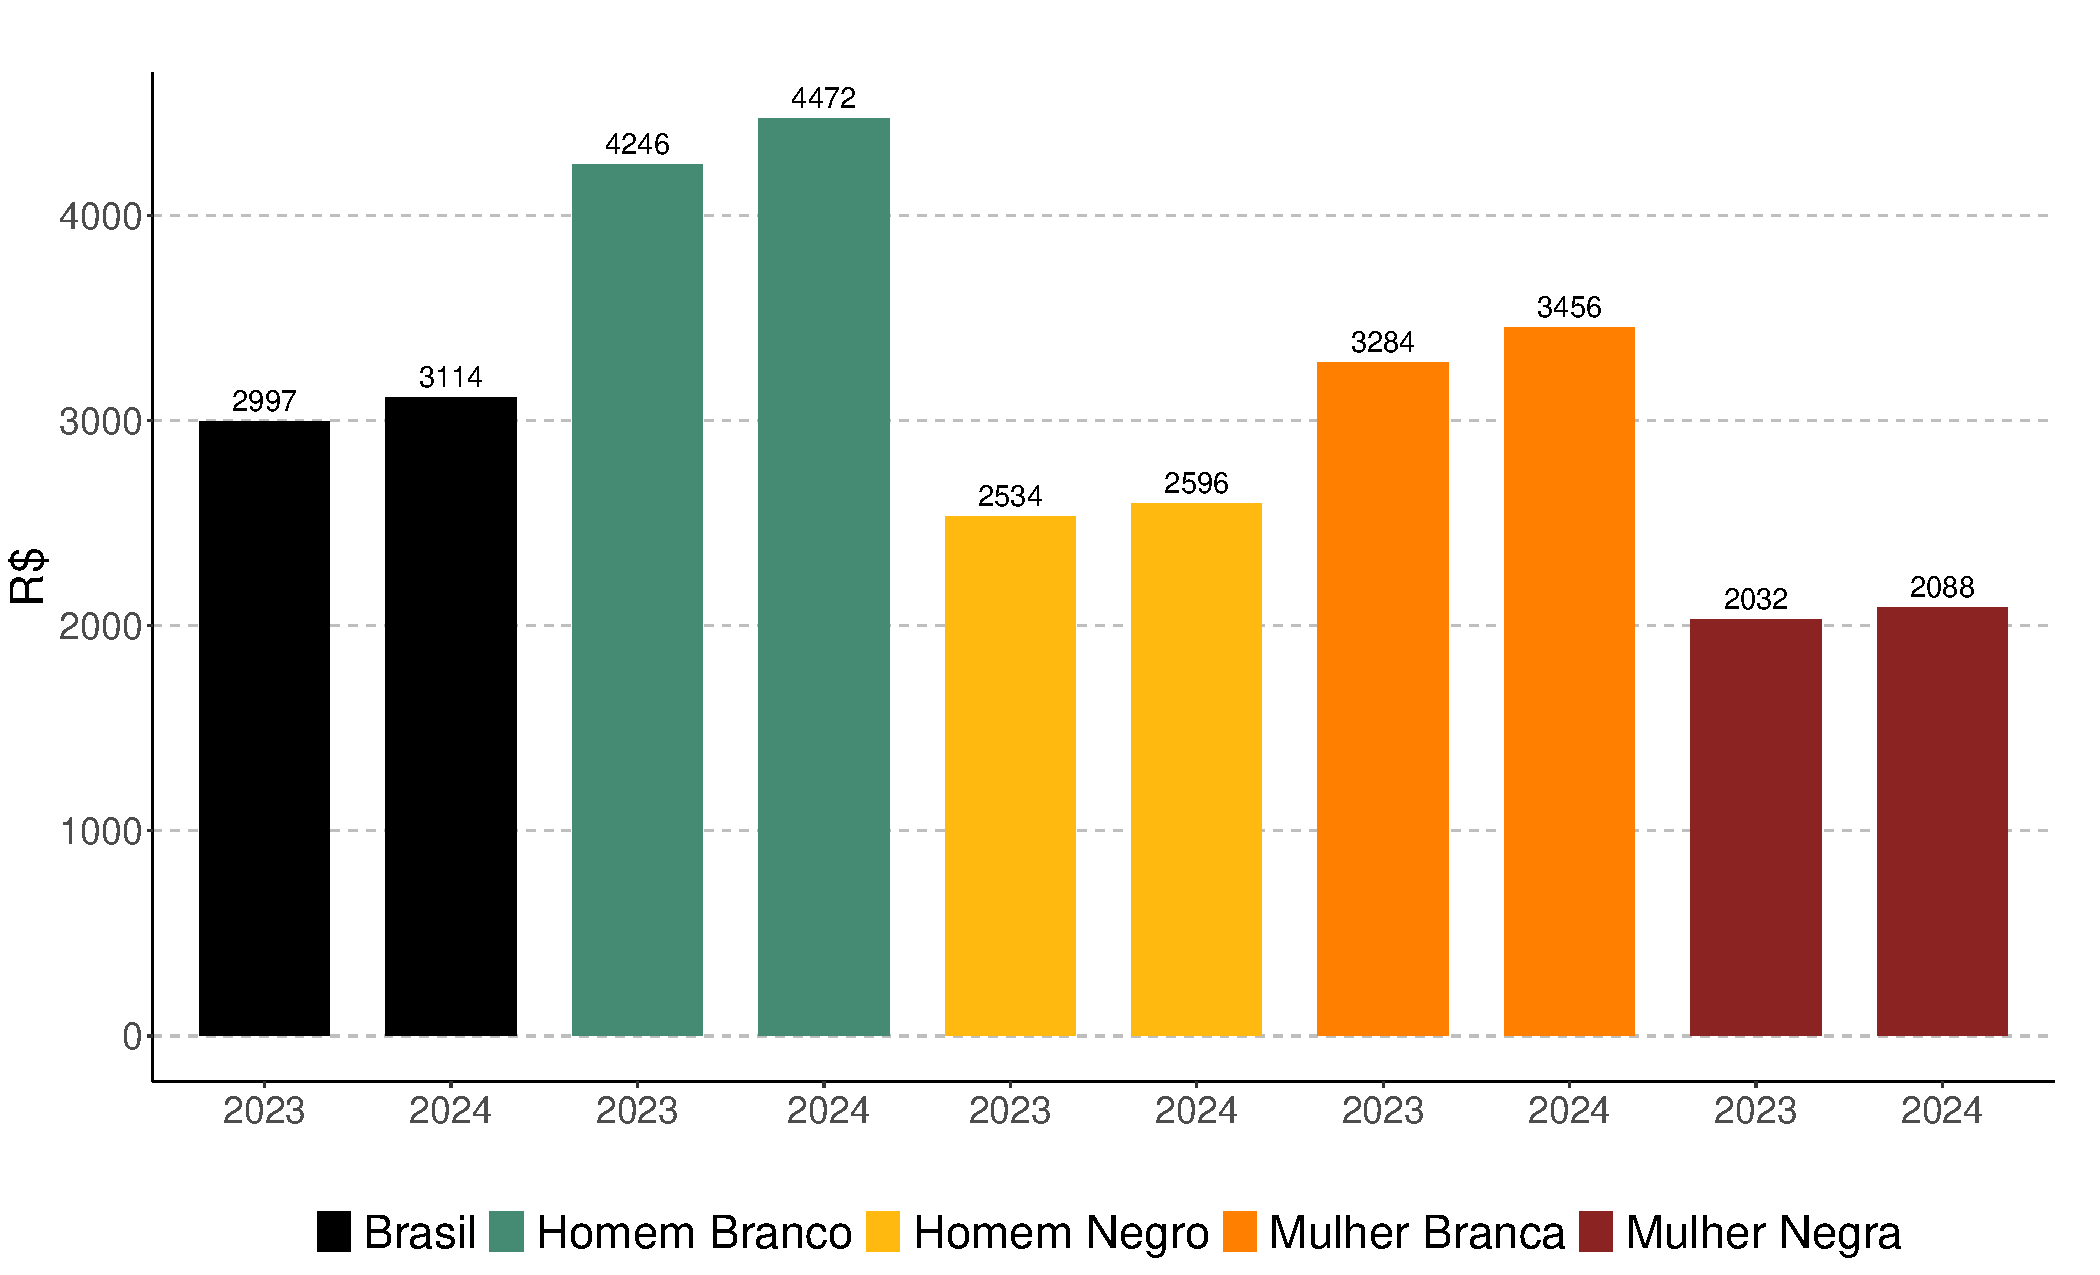
\includegraphics[width = 0.75\textwidth]{figures_output/rendimento_habitual.pdf}
		\end{figure}
	\end{frame}			
	
	\begin{frame}{Desigualdade Salarial}
		\begin{figure}
			\centering
			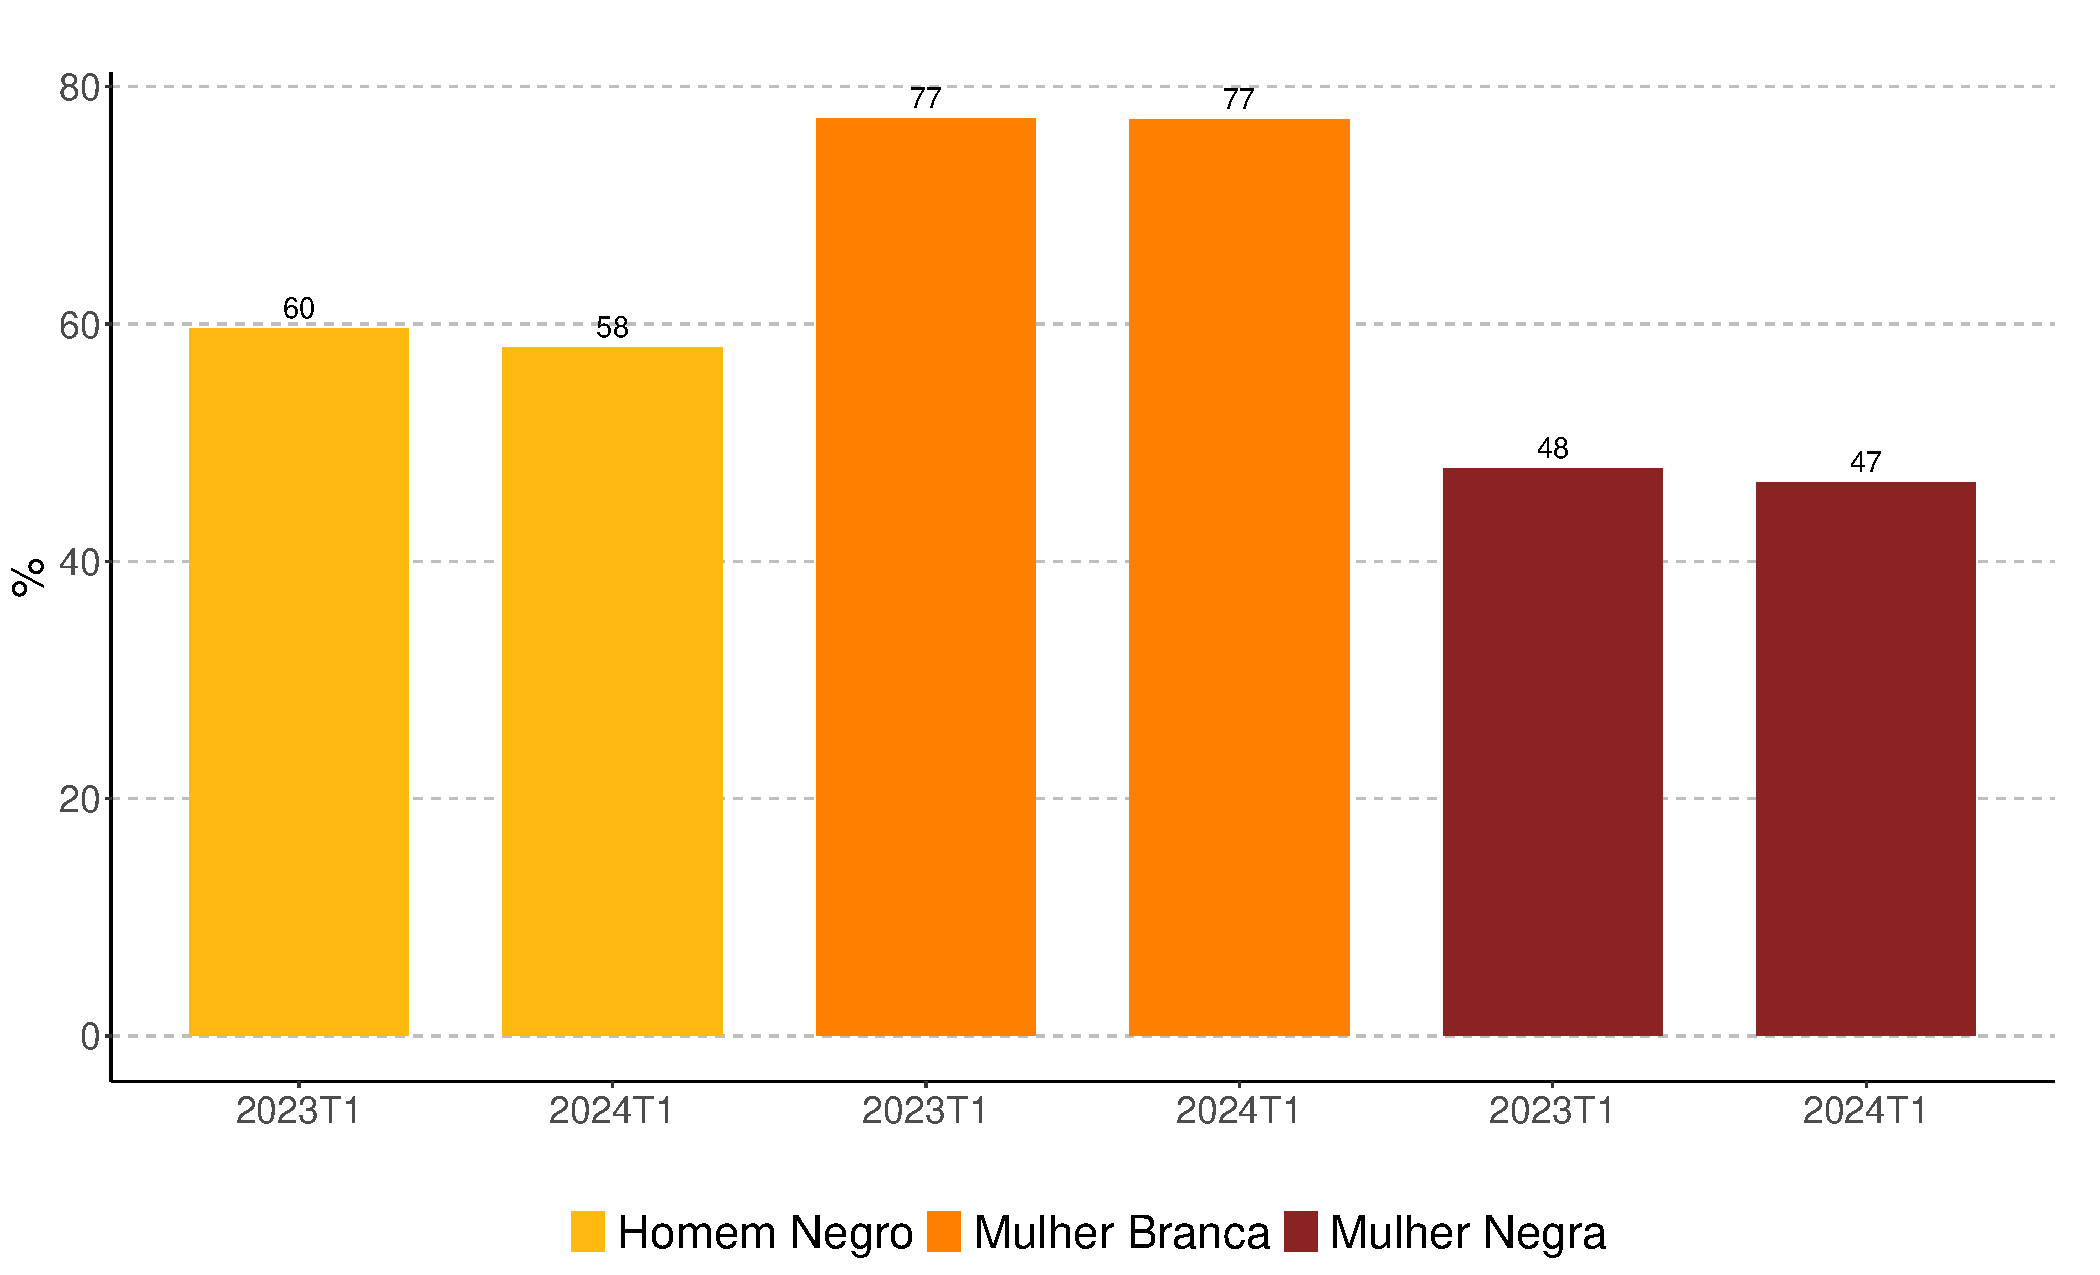
\includegraphics[width = 0.75\textwidth]{figures_output/frac_rendimento_habitual.pdf}
		\end{figure}
	\end{frame}			
	
	\begin{frame}{Rendimento Habitual Médio de Todos os Trabalhos}
		\begin{figure}
			\centering
			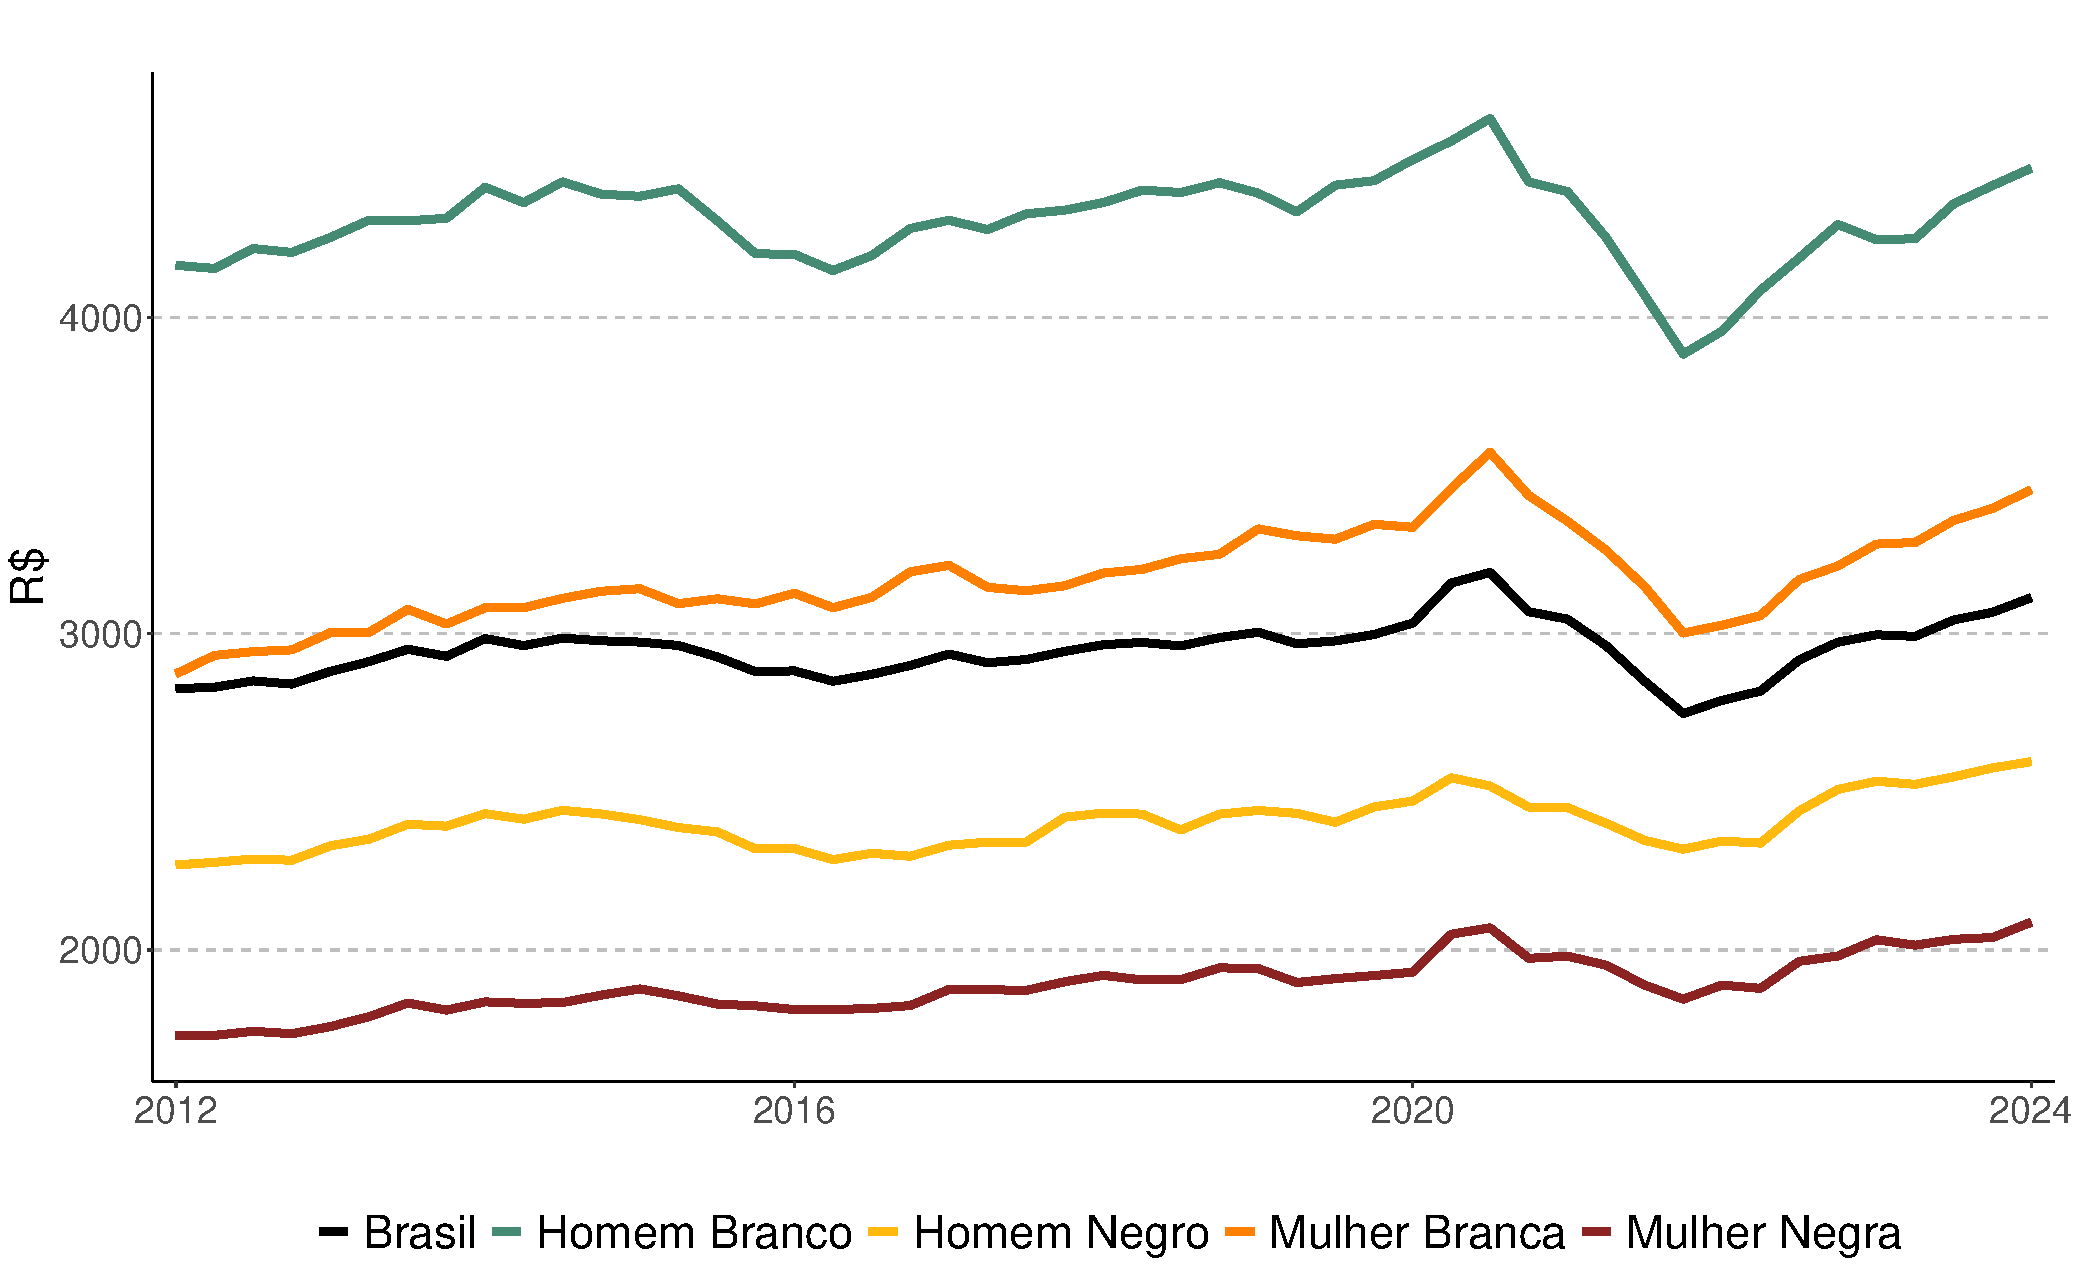
\includegraphics[width = 0.75\textwidth]{figures_output/rendimento_habitual_br_gen_raca.pdf}
		\end{figure}
	\end{frame}	
	
	\begin{frame}{Desemprego Recente}
		\begin{figure}
			\centering
			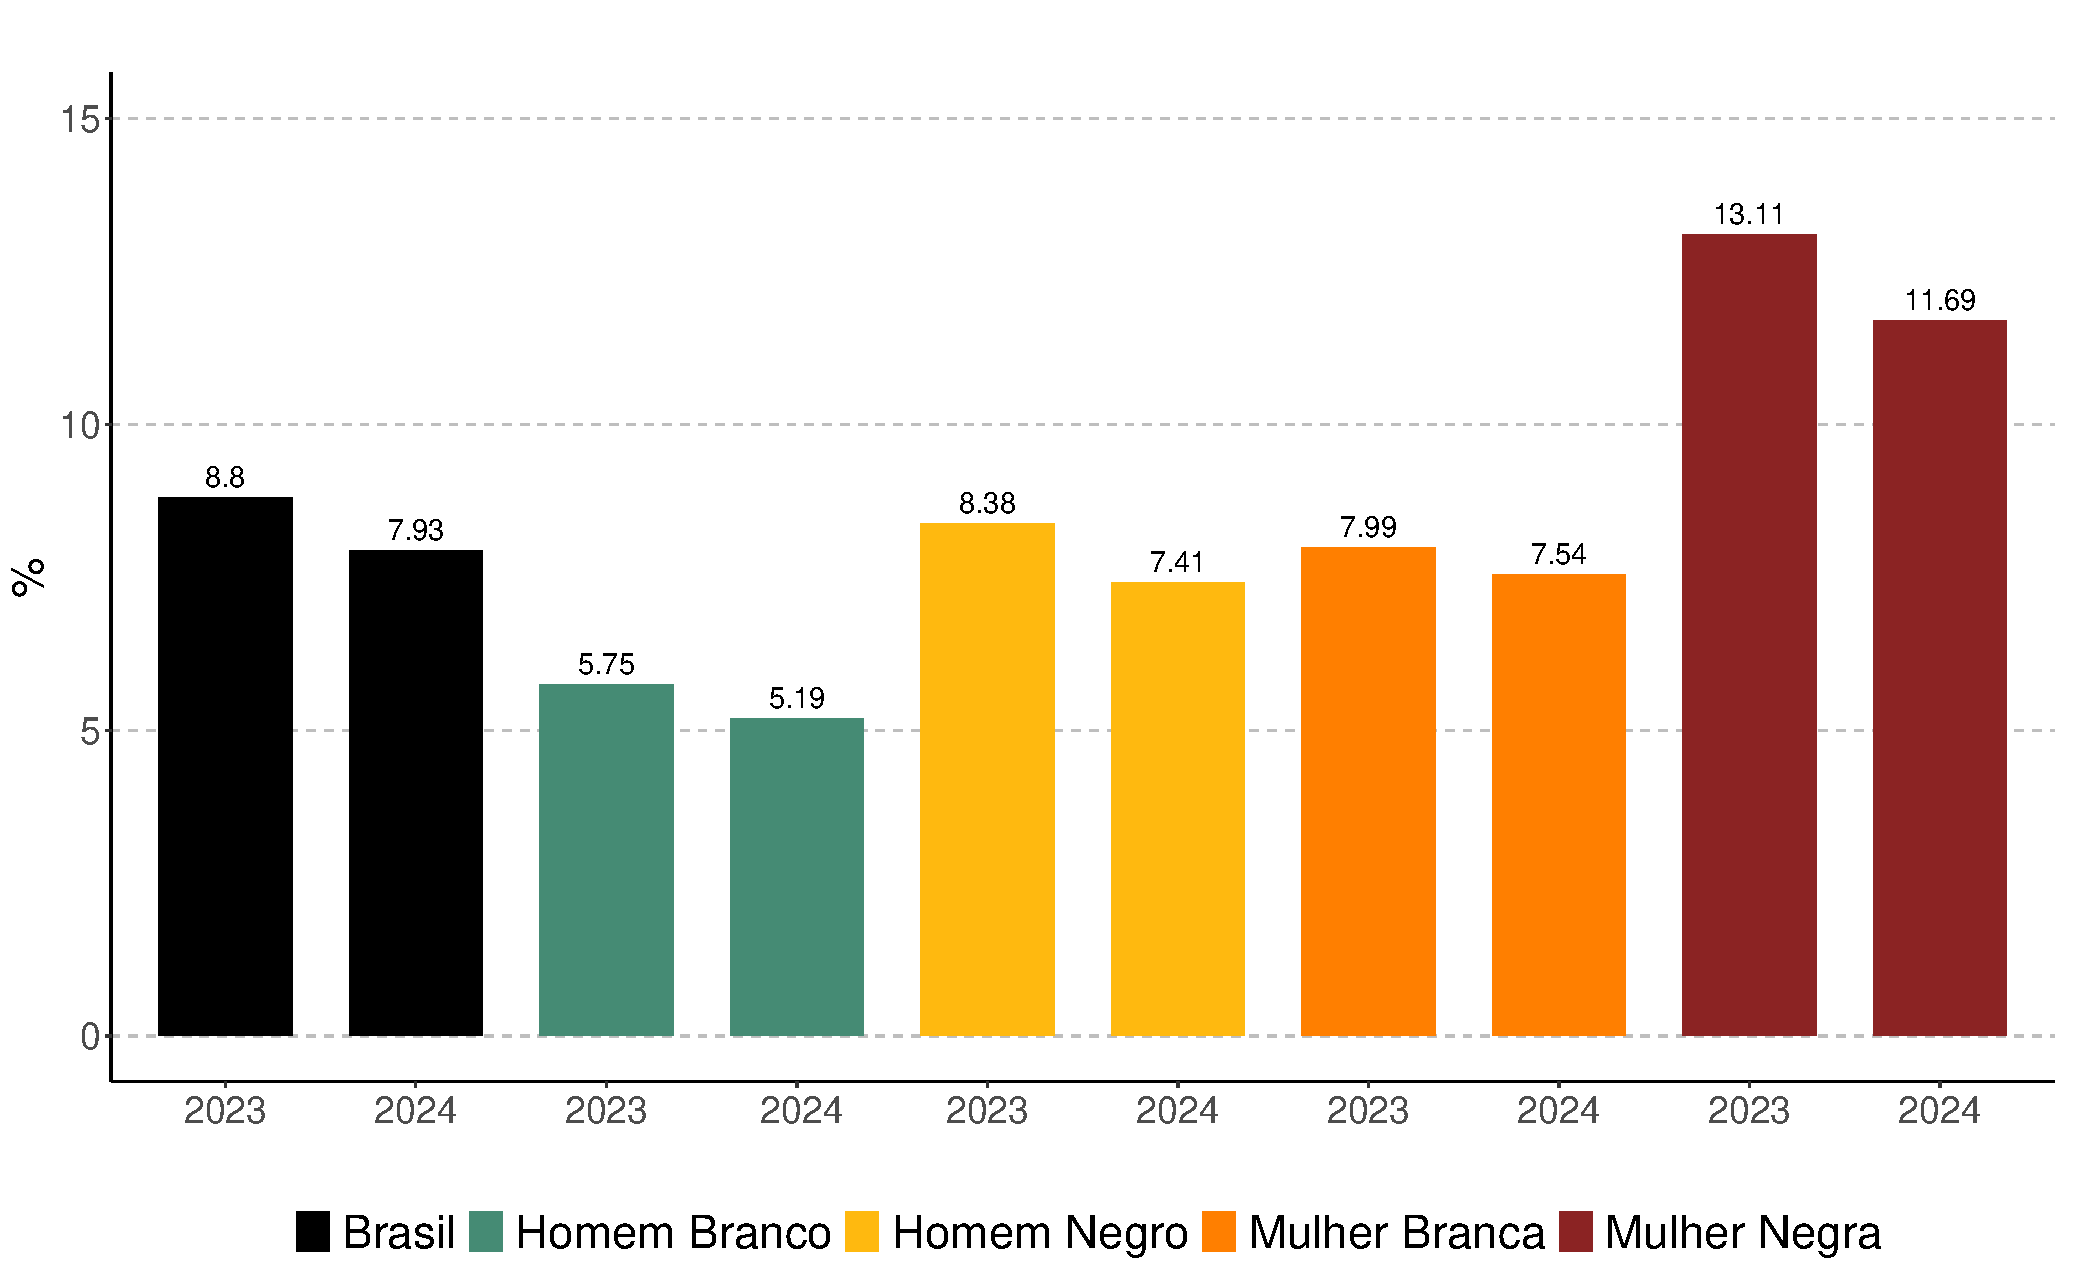
\includegraphics[width = 0.75\textwidth]{figures_output/unemp.pdf}
		\end{figure}
	\end{frame}
	
	\begin{frame}{Probabilidade de estar Desempregado}
		\begin{figure}
			\centering
			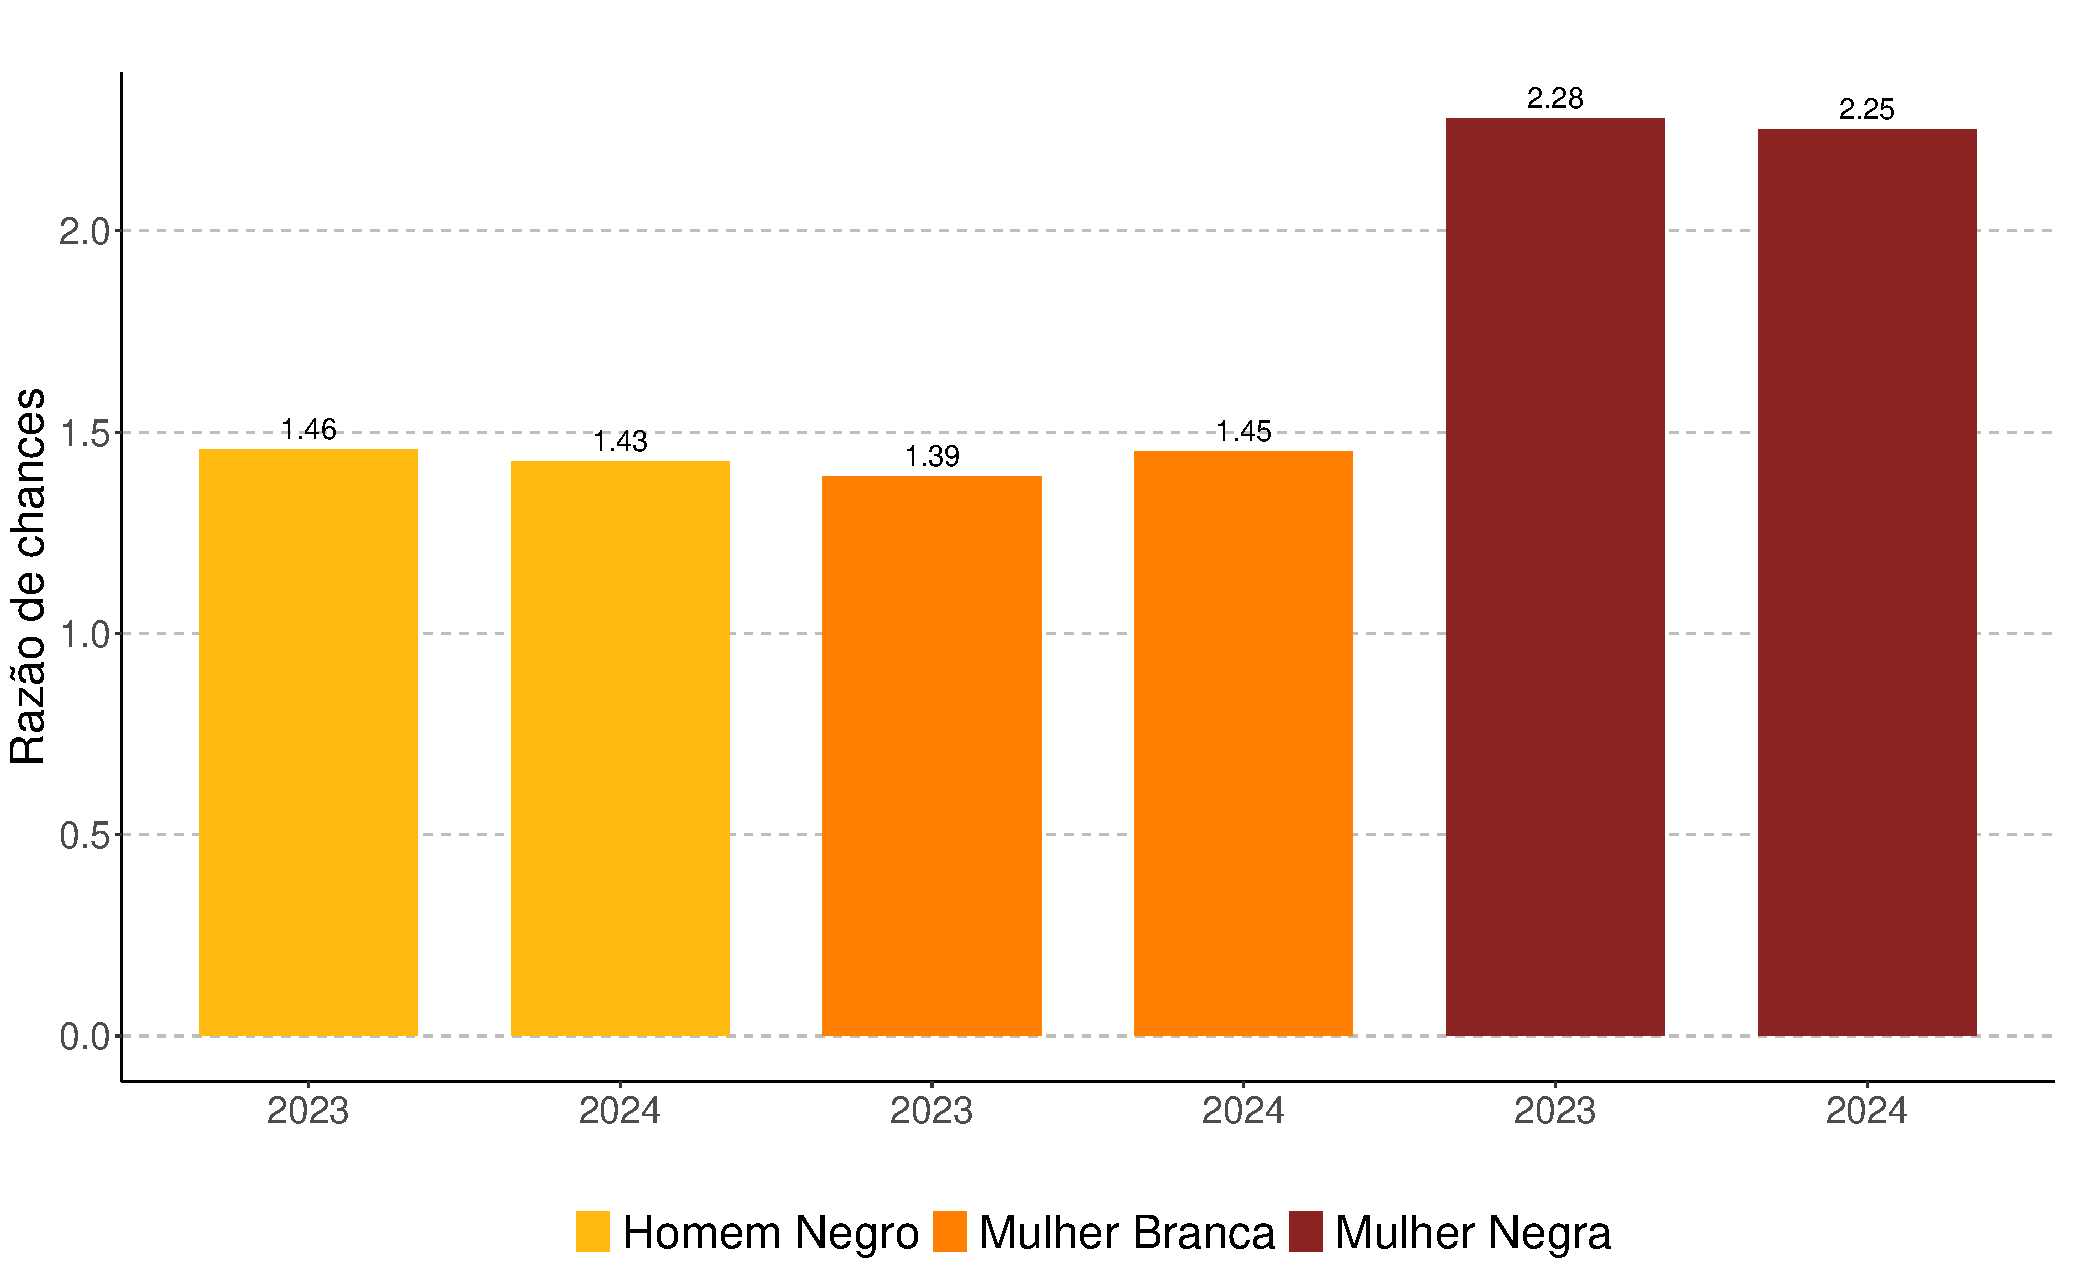
\includegraphics[width = 0.75\textwidth]{figures_output/frac_unemp.pdf}
		\end{figure}
	\end{frame}
	
	\begin{frame}{Taxa de Desemprego}
		\begin{figure}
			\centering
			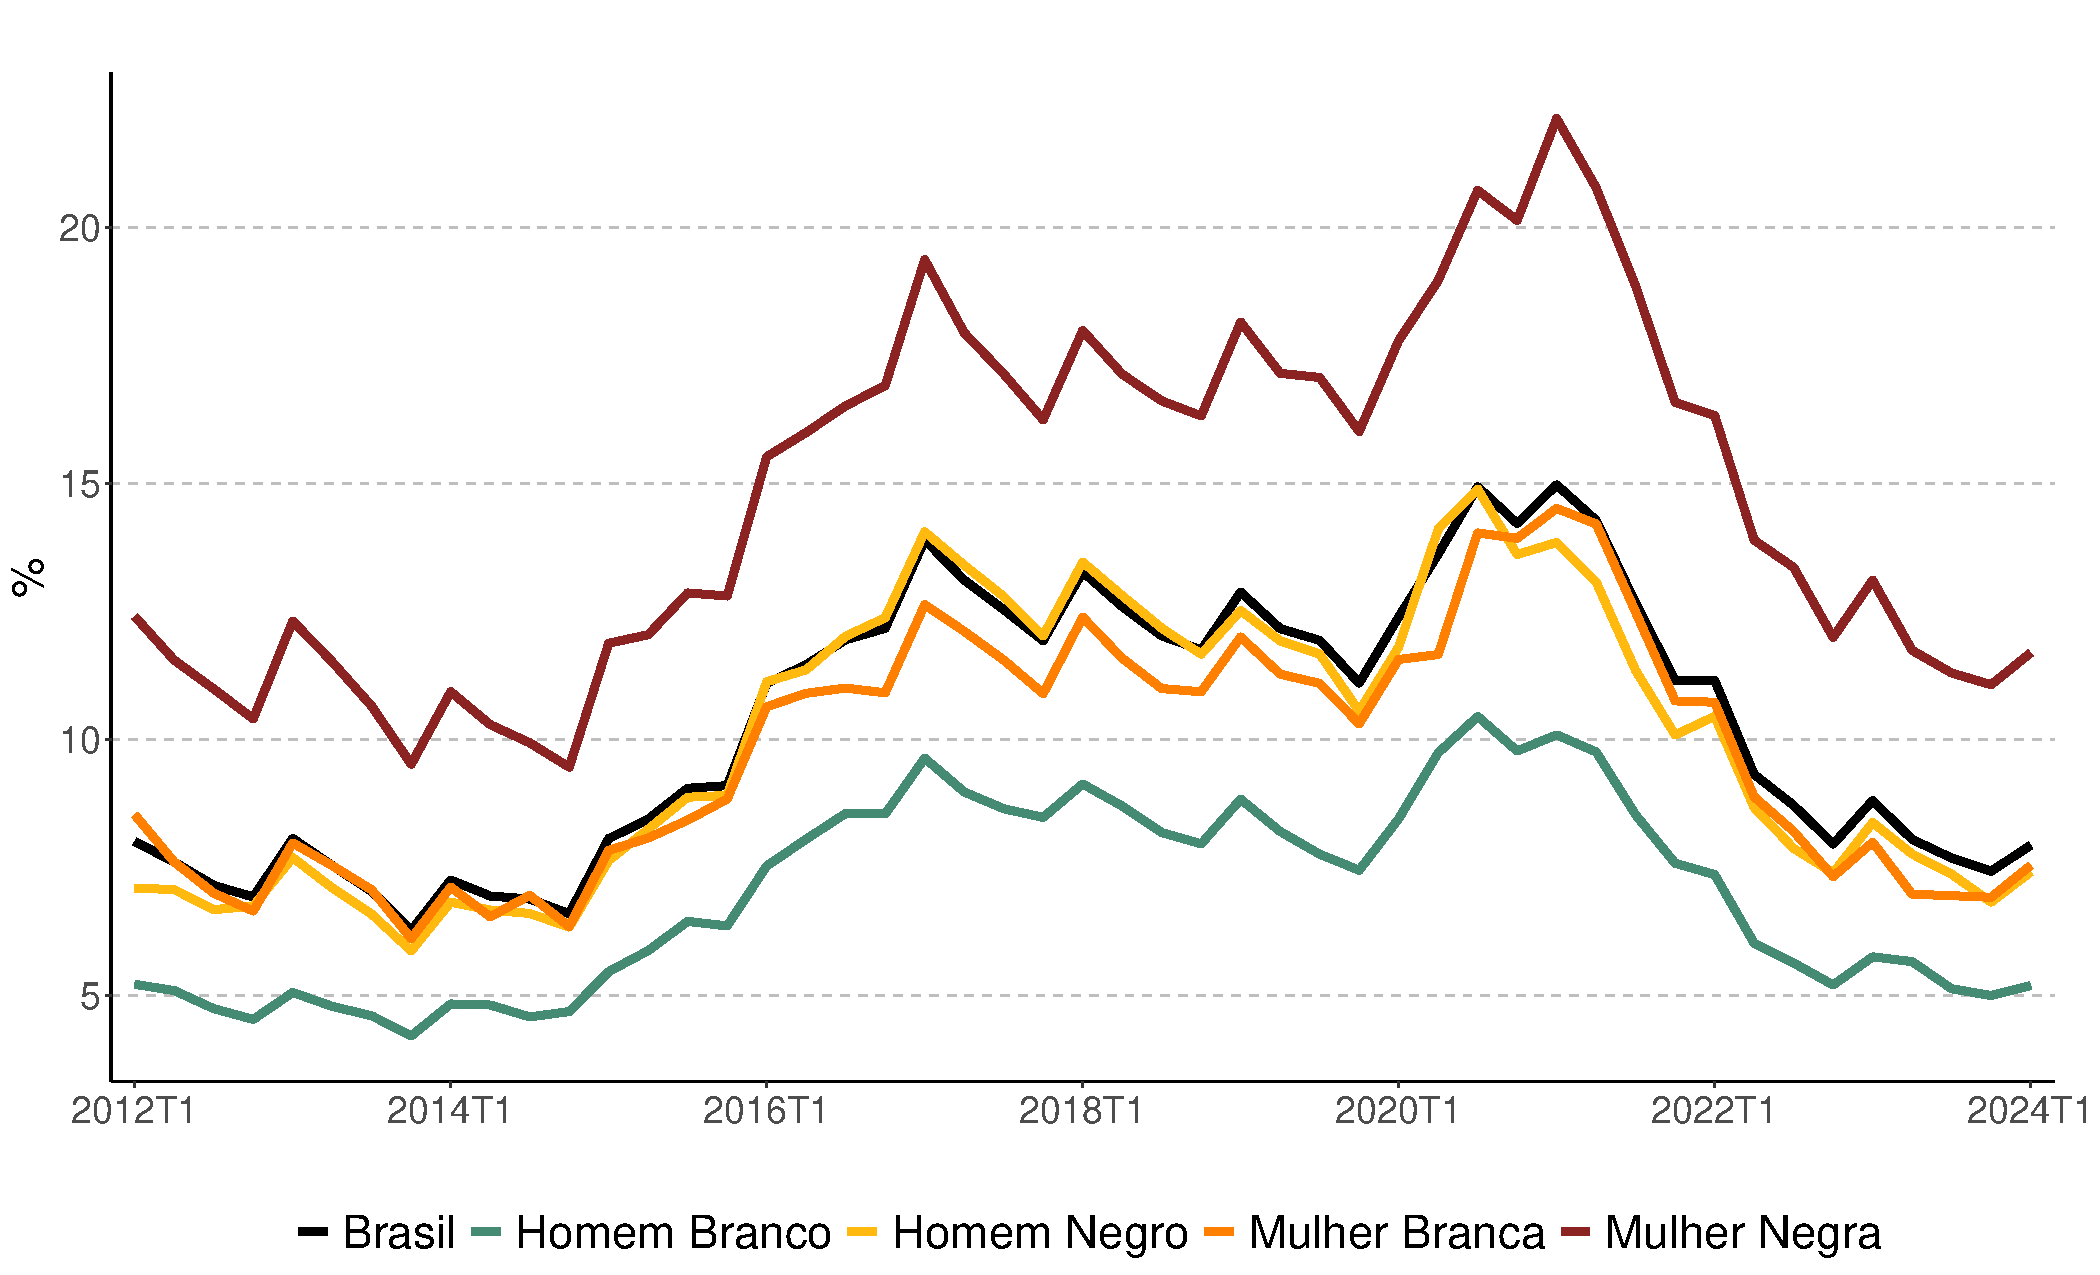
\includegraphics[width = 0.75\textwidth]{figures_output/unemp_br_gen_raca.pdf}
		\end{figure}
	\end{frame}			
	
	\begin{frame}{Desigualdade na PEA}
		\begin{figure}
			\centering
			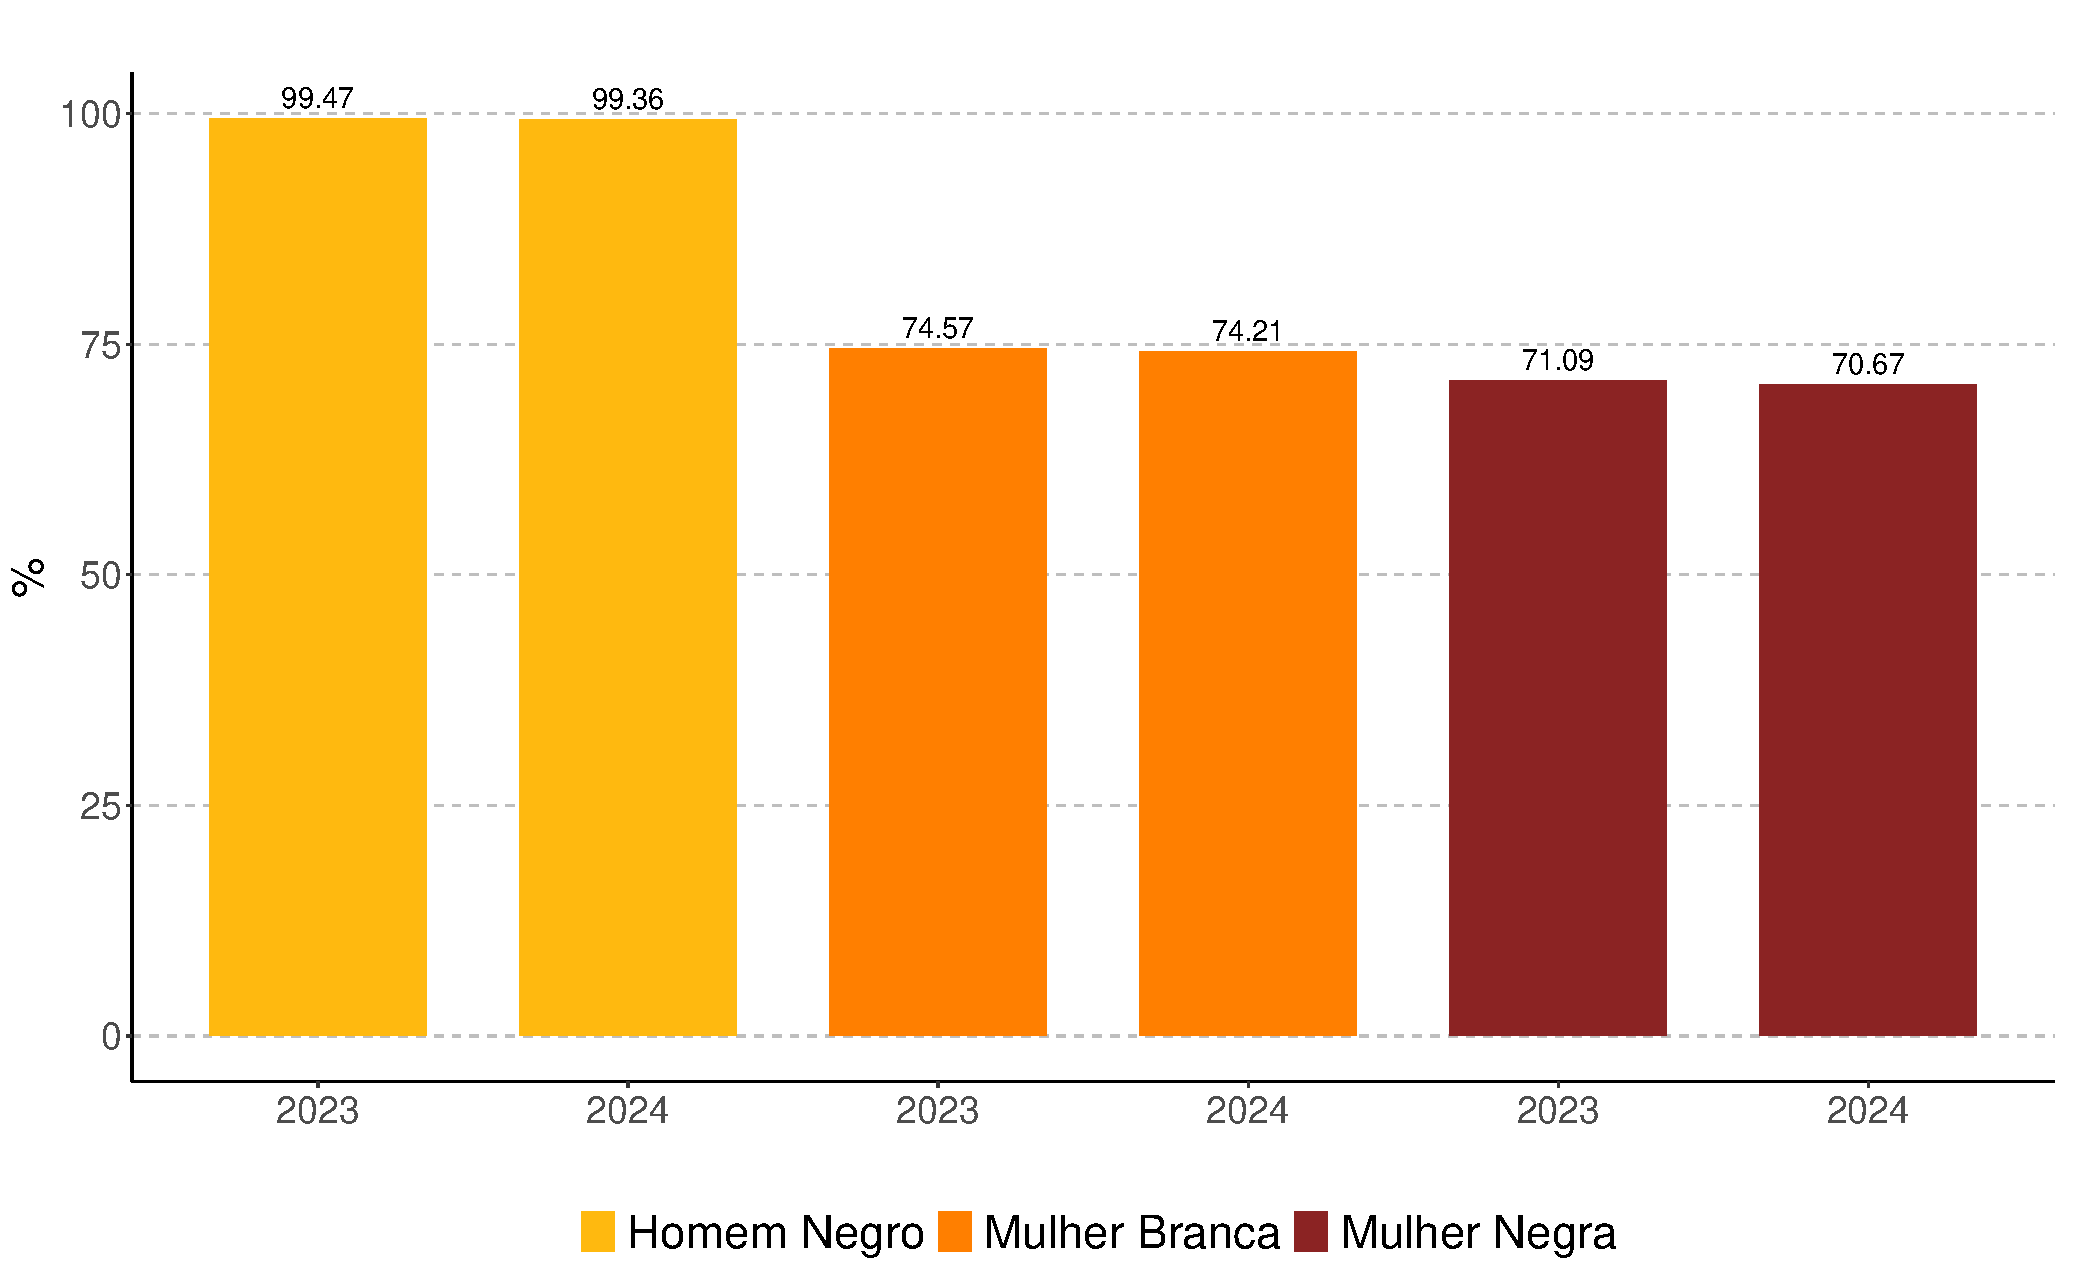
\includegraphics[width = 0.75\textwidth]{figures_output/frac_pea.pdf}
		\end{figure}
	\end{frame}	
	
	\begin{frame}{PEA Recente}
		\begin{figure}
			\centering
			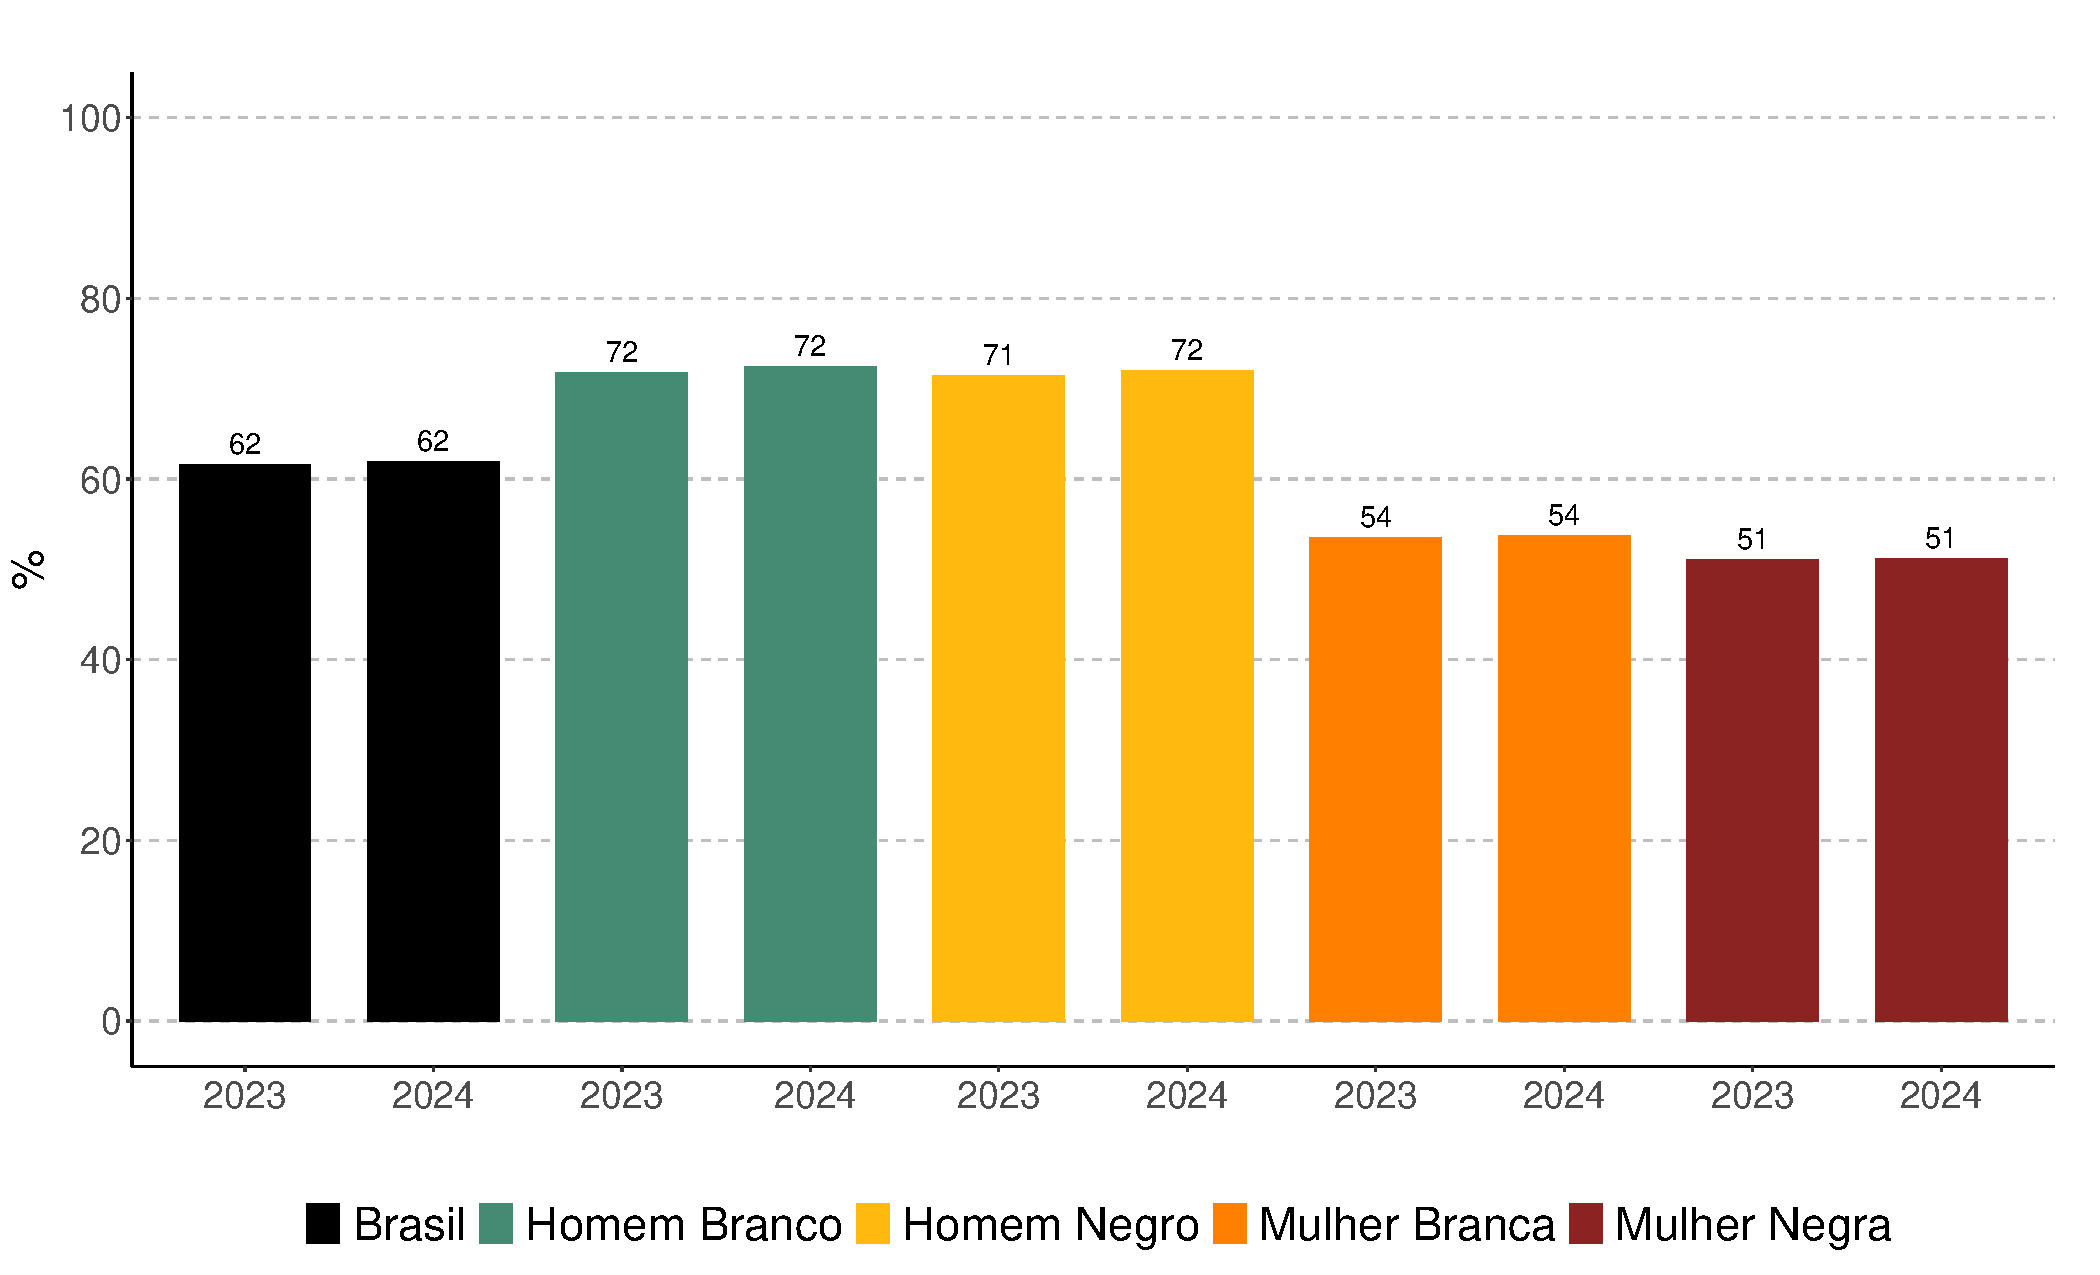
\includegraphics[width = 0.75\textwidth]{figures_output/pea.pdf}
		\end{figure}
	\end{frame}	
	
	\begin{frame}{PEA Recente - 25 a 54 anos}
		\begin{figure}
			\centering
			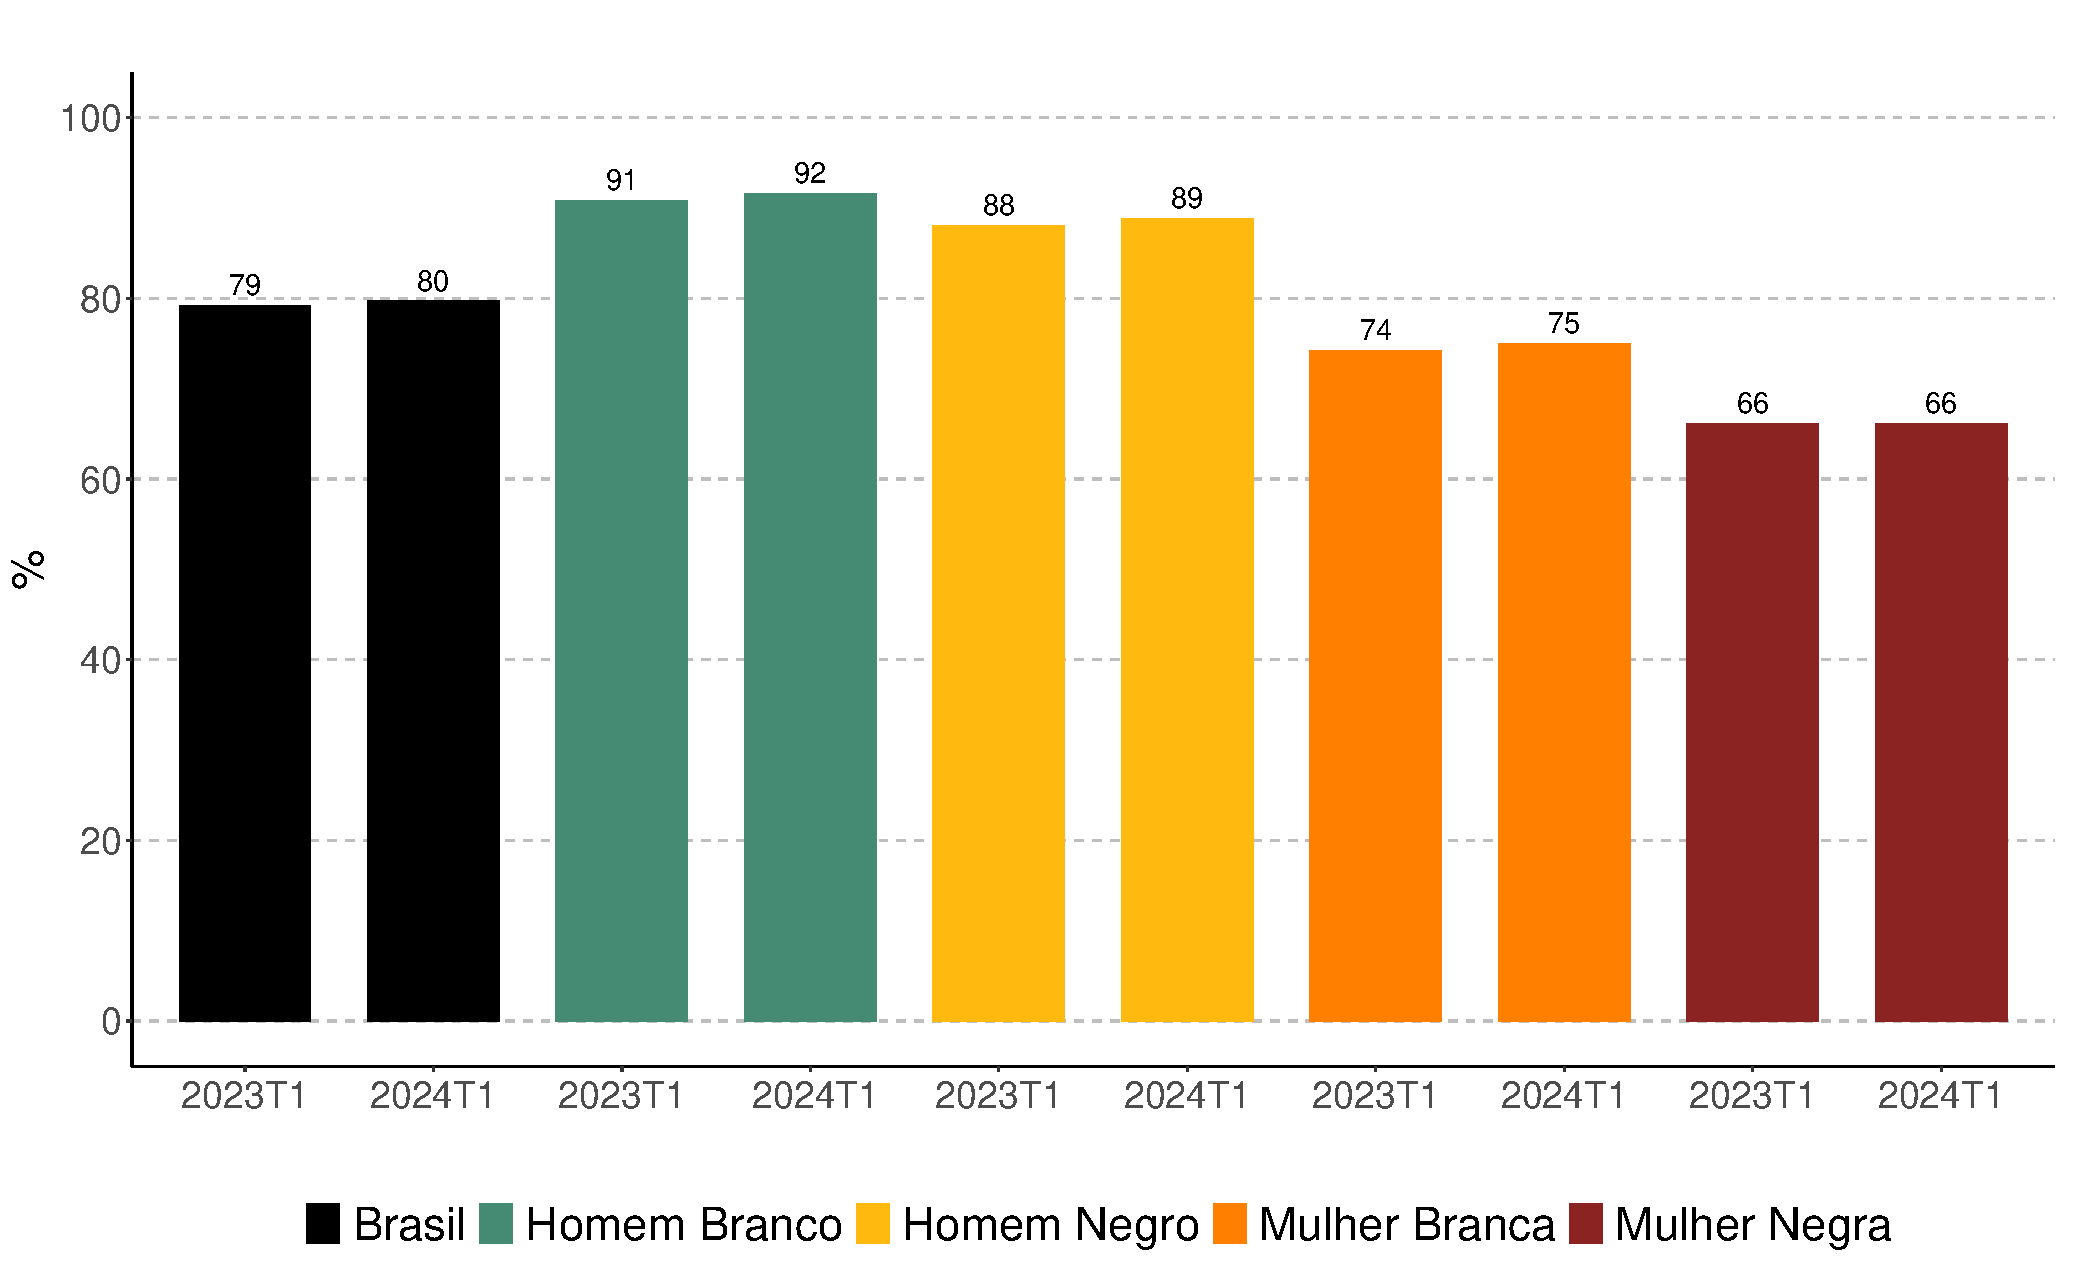
\includegraphics[width = 0.75\textwidth]{figures_output/pea_adult.pdf}
		\end{figure}
	\end{frame}	
	
	\begin{frame}{PEA}
		\begin{figure}
			\centering
			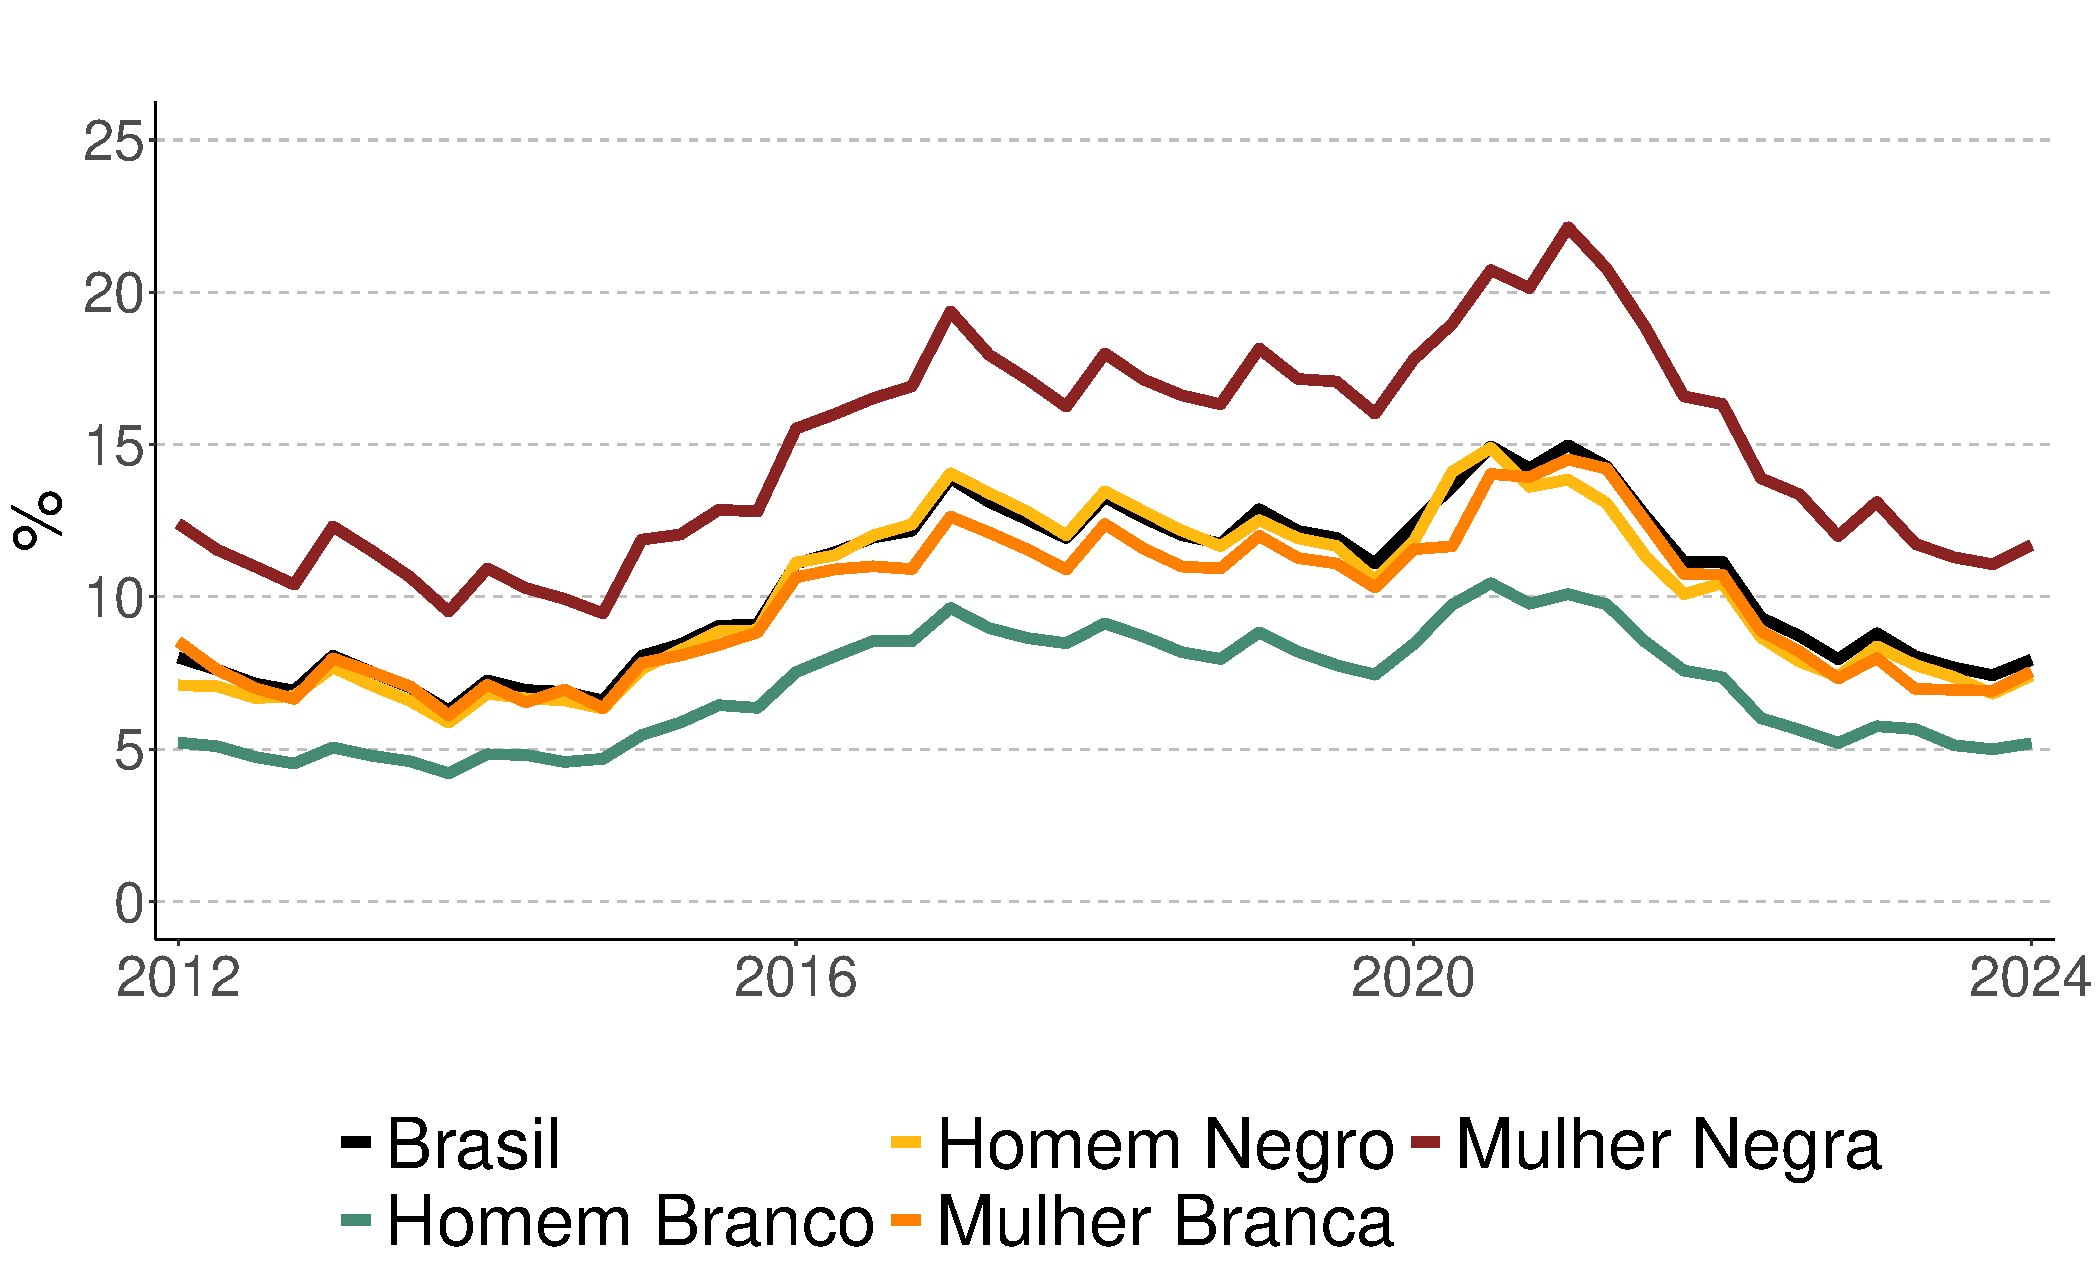
\includegraphics[width = 0.75\textwidth]{figures_output/pea_br_gen_raca.pdf}
		\end{figure}
	\end{frame}	
	
	
	\begin{frame}{Gini}
		\begin{figure}
			\centering
			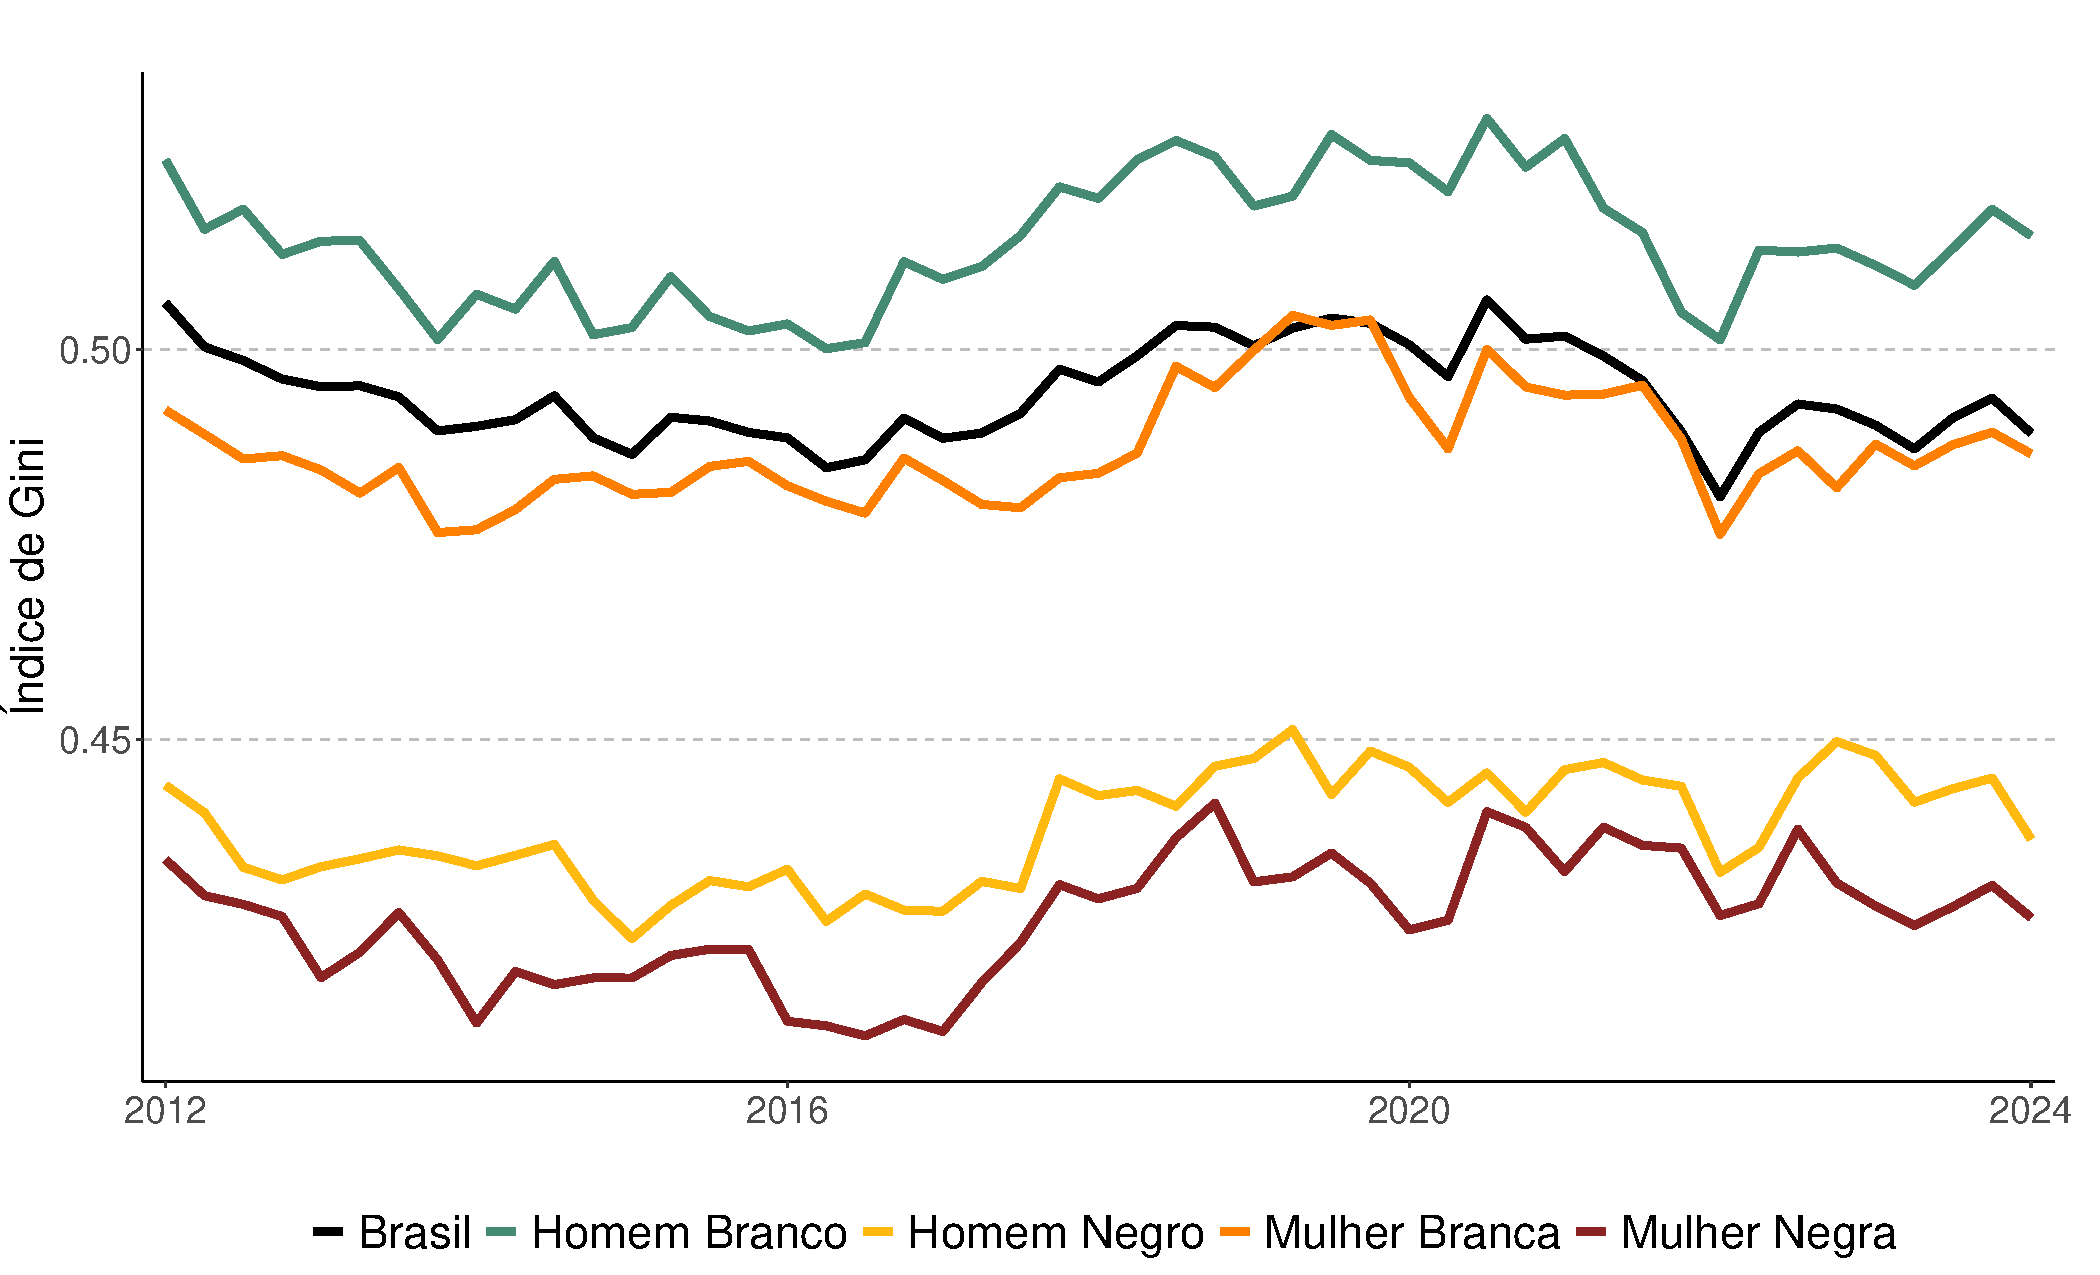
\includegraphics[width = 0.75\textwidth]{figures_output/gini_br_gen_raca.pdf}
		\end{figure}
	\end{frame}
	
	\begin{frame}{Um por cento mais pobre e mais rico}
		\begin{figure}
			\centering
			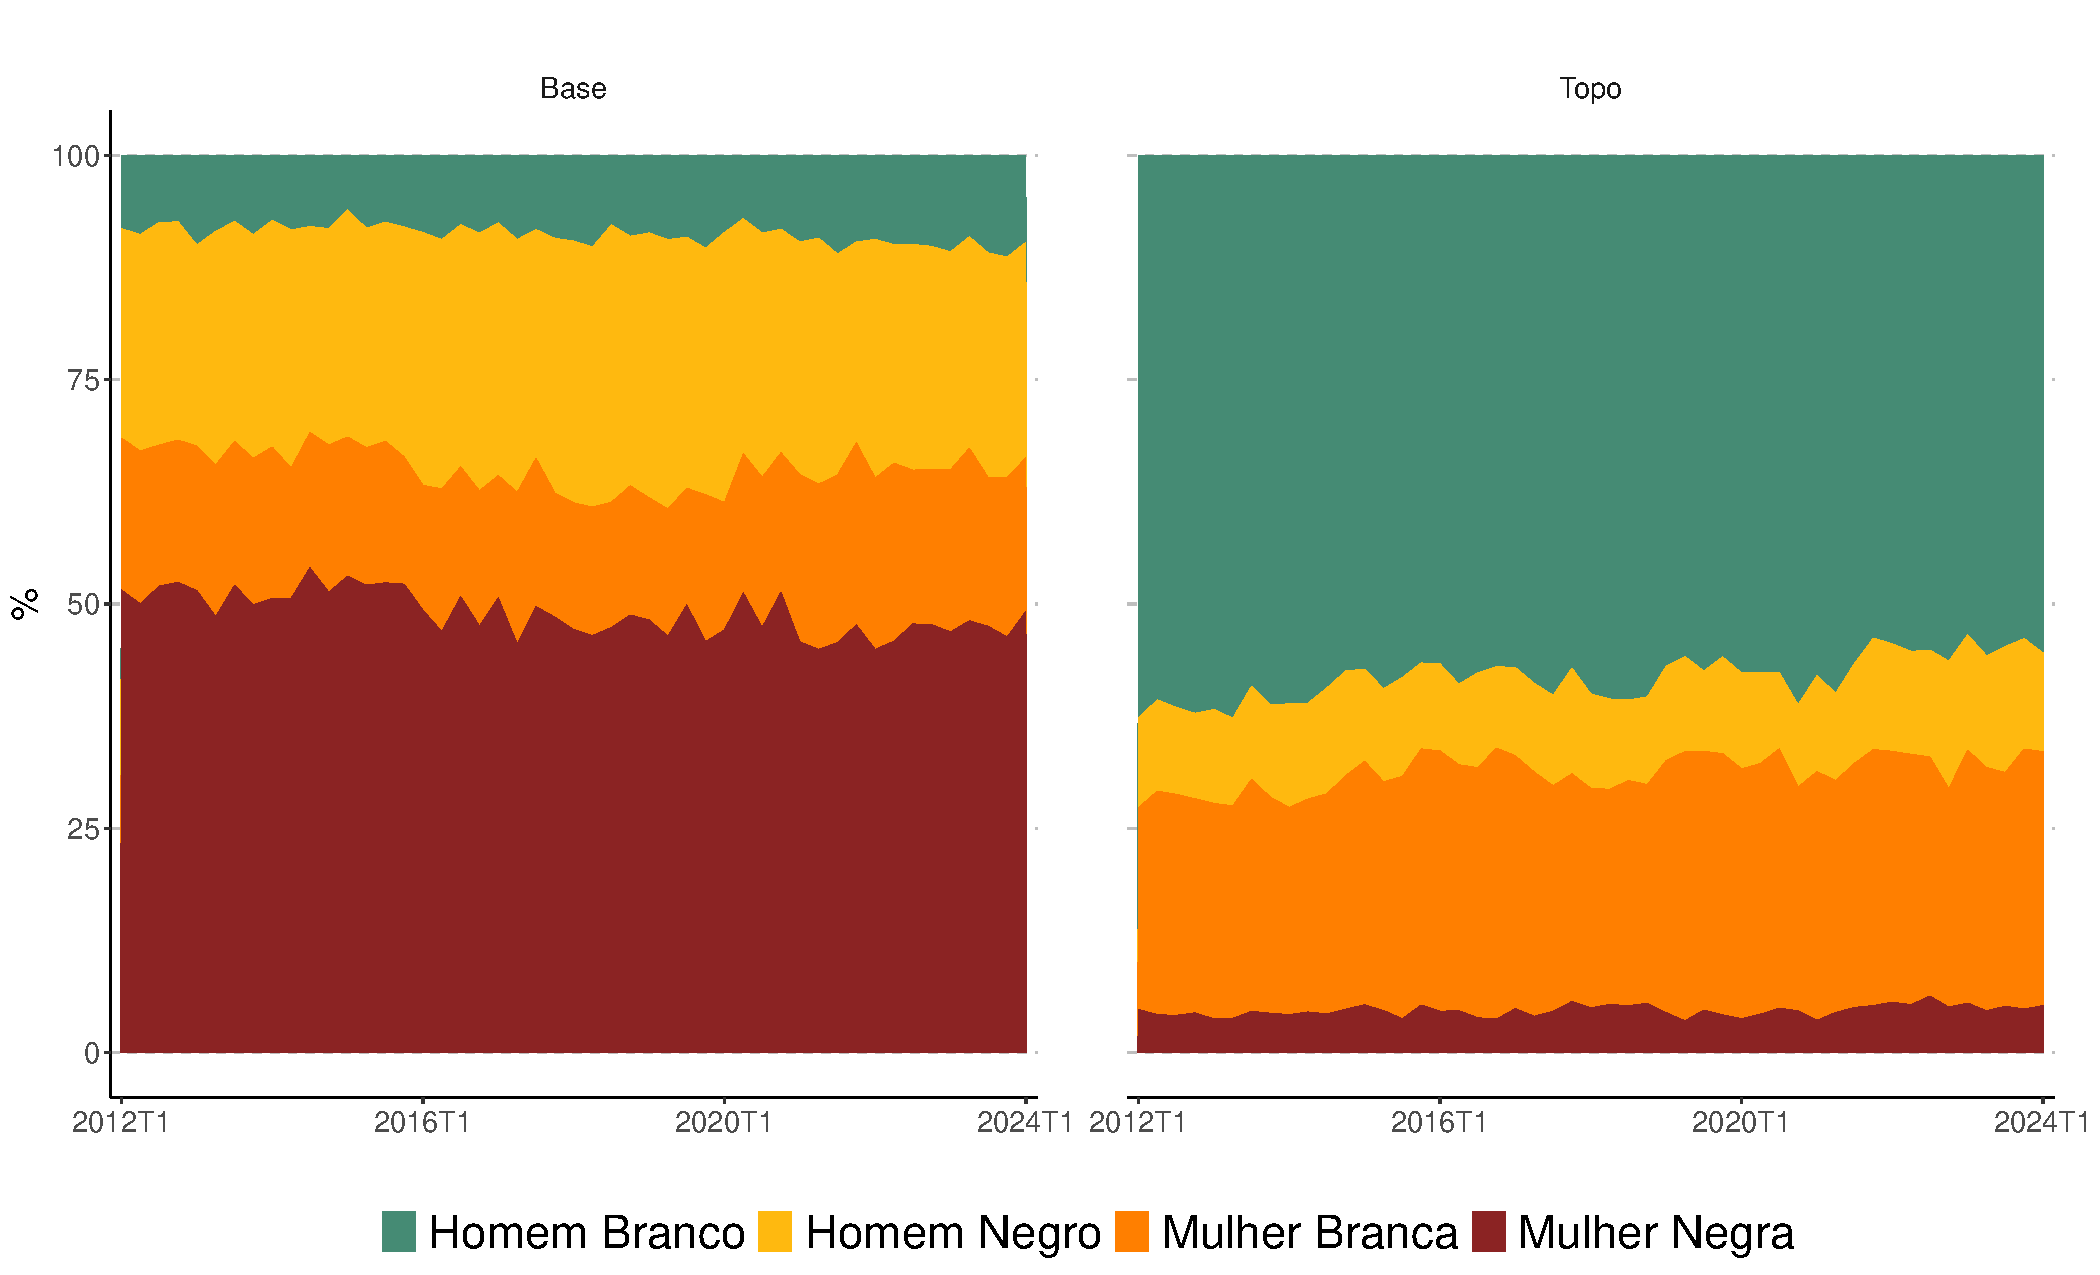
\includegraphics[width = 0.75\textwidth]{figures_output/base_topo_1.pdf}
		\end{figure}
	\end{frame}
	
		\begin{frame}{Os cinco por cento mais pobre e mais rico}
		\begin{figure}
			\centering
			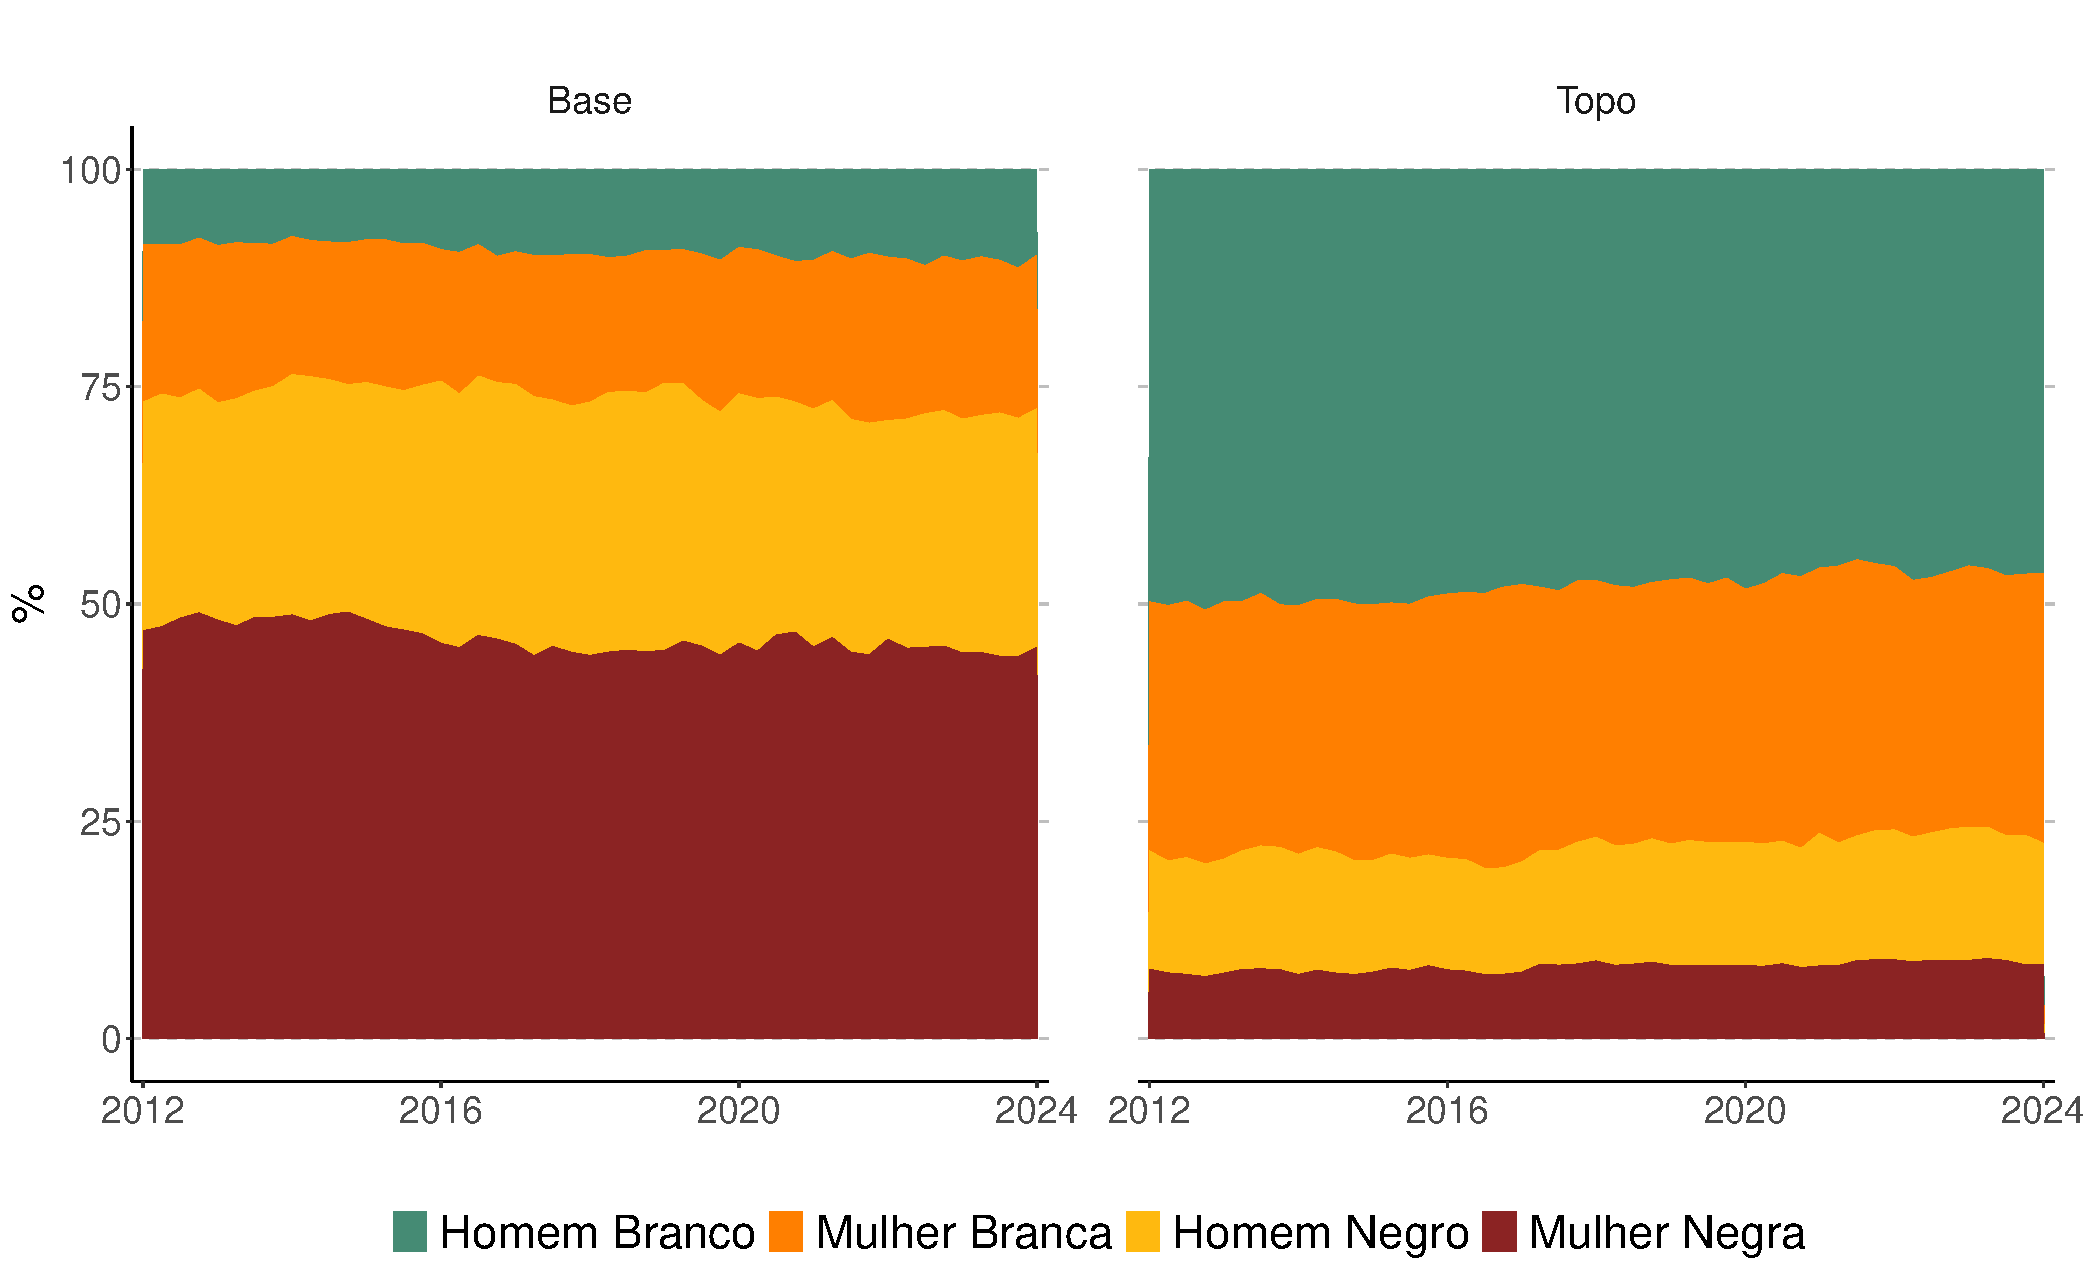
\includegraphics[width = 0.75\textwidth]{figures_output/base_topo_5.pdf}
		\end{figure}
	\end{frame}
	
		\begin{frame}{Os dez por cento mais pobre e mais rico}
		\begin{figure}
			\centering
			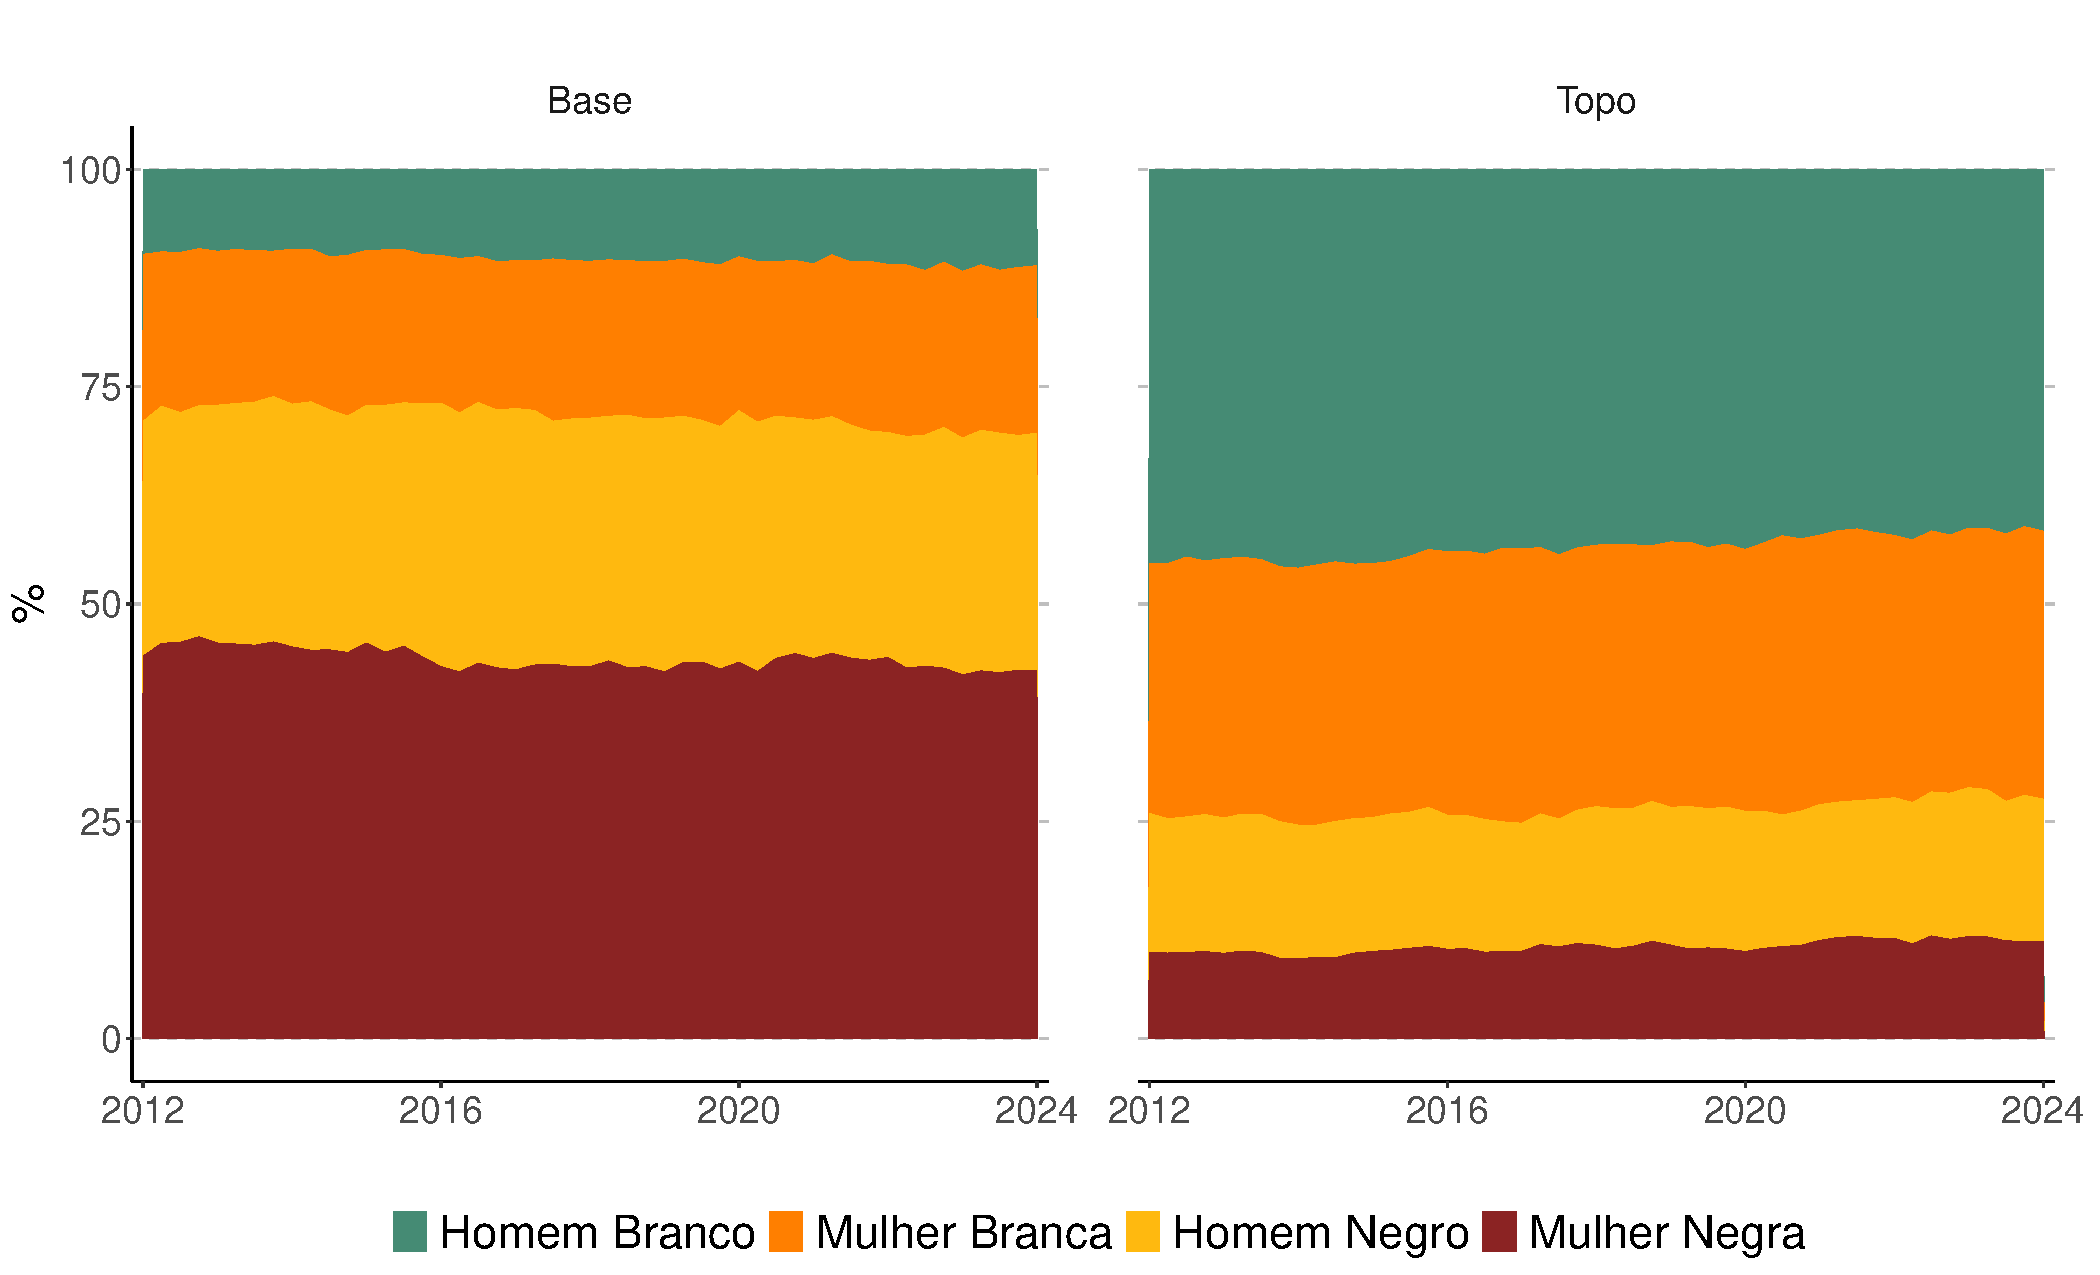
\includegraphics[width = 0.75\textwidth]{figures_output/base_topo_10.pdf}
		\end{figure}
	\end{frame}
		
		\begin{frame}{Um por cento mais pobre e mais rico}
		\begin{figure}
			\centering
			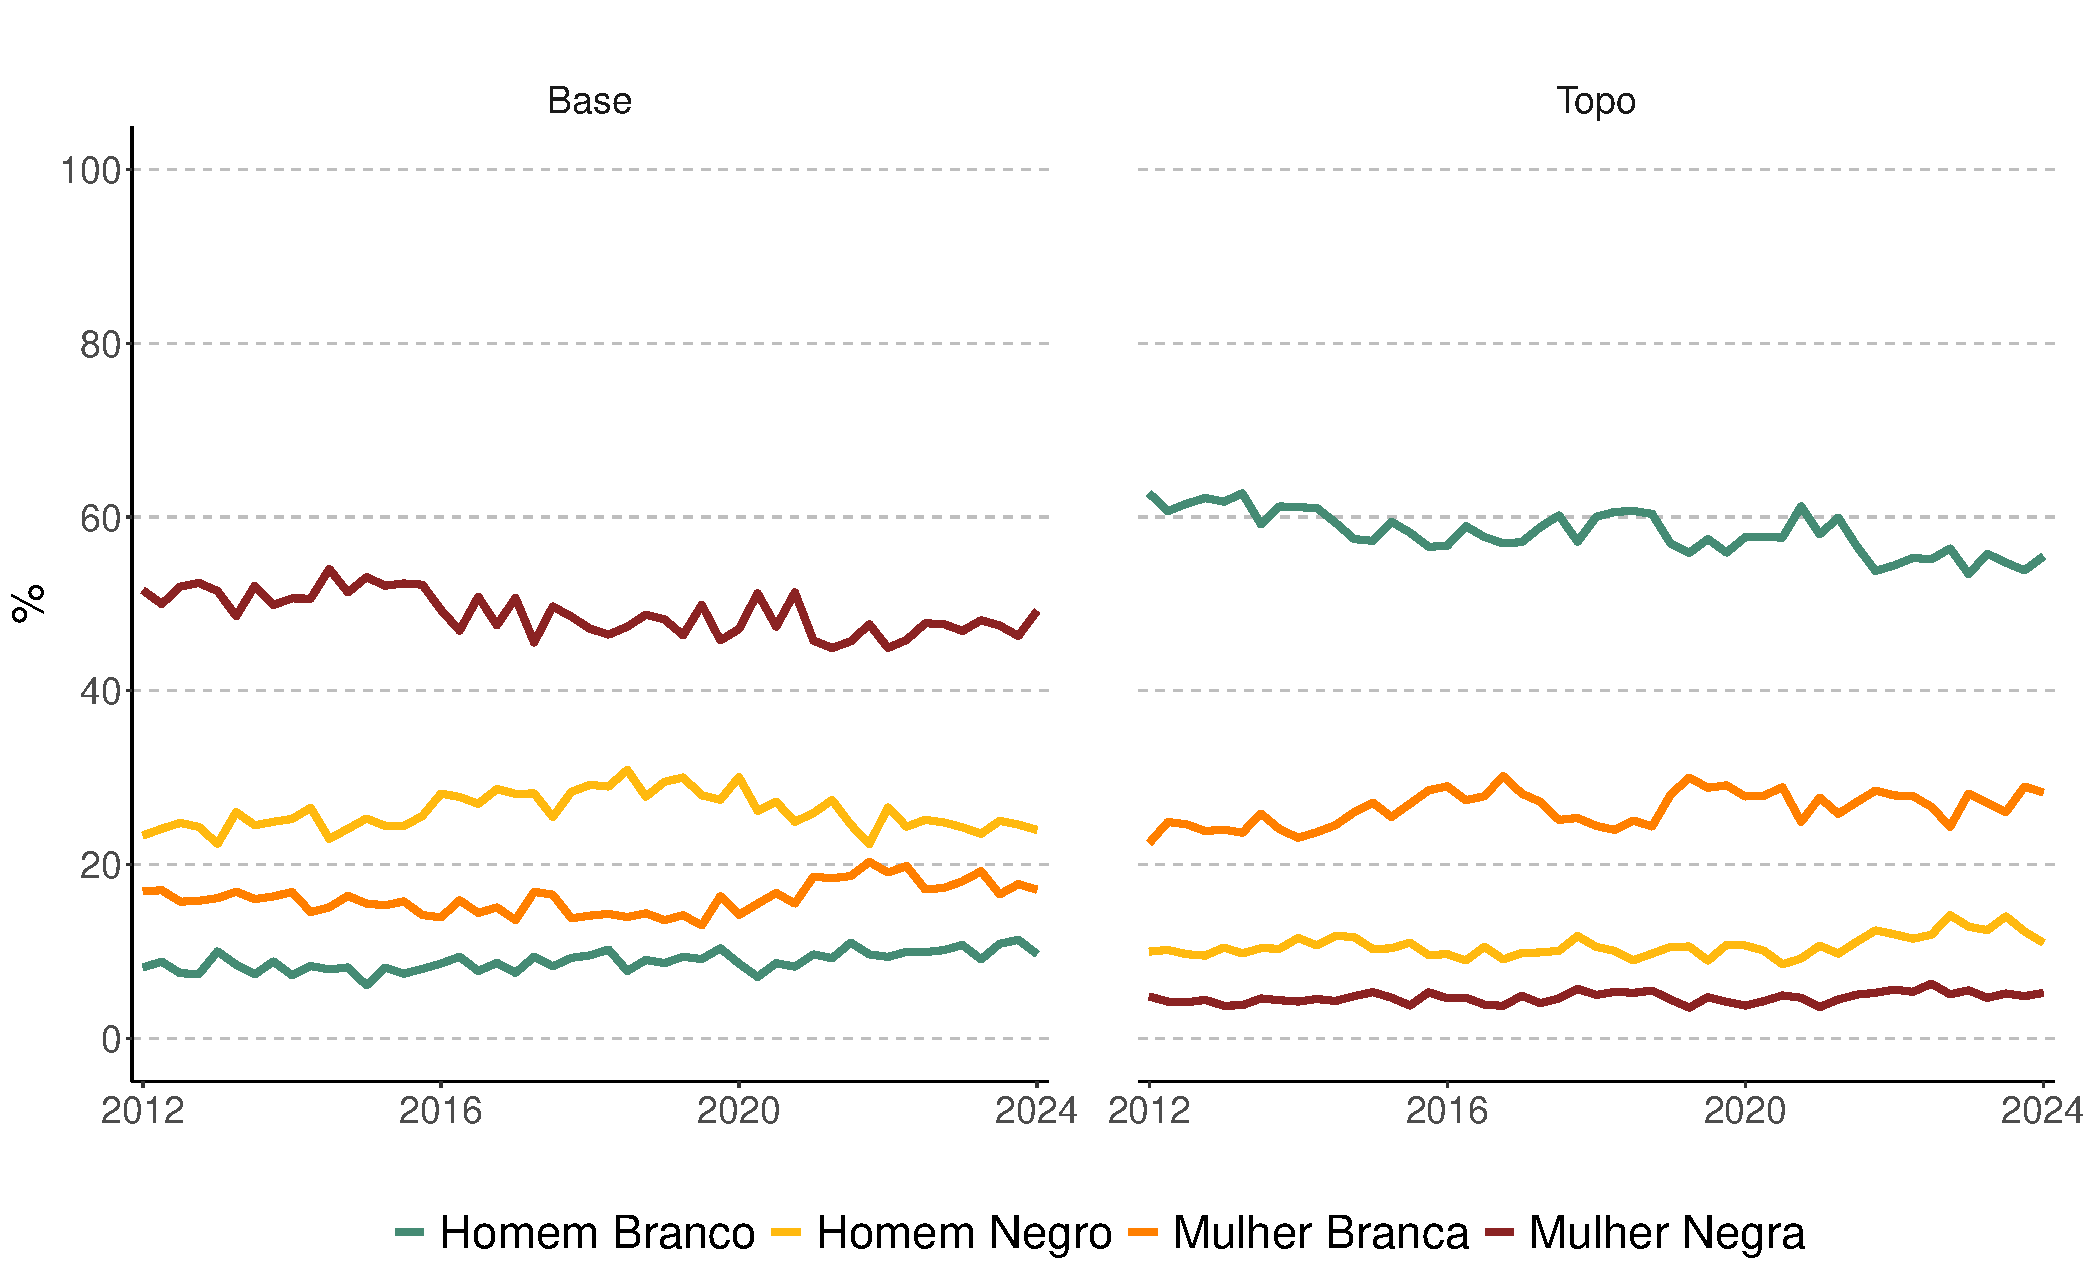
\includegraphics[width = 0.75\textwidth]{figures_output/base_topo_1_linha.pdf}
		\end{figure}
	\end{frame}
	
	\begin{frame}{Os cinco por cento mais pobre e mais rico}
		\begin{figure}
			\centering
			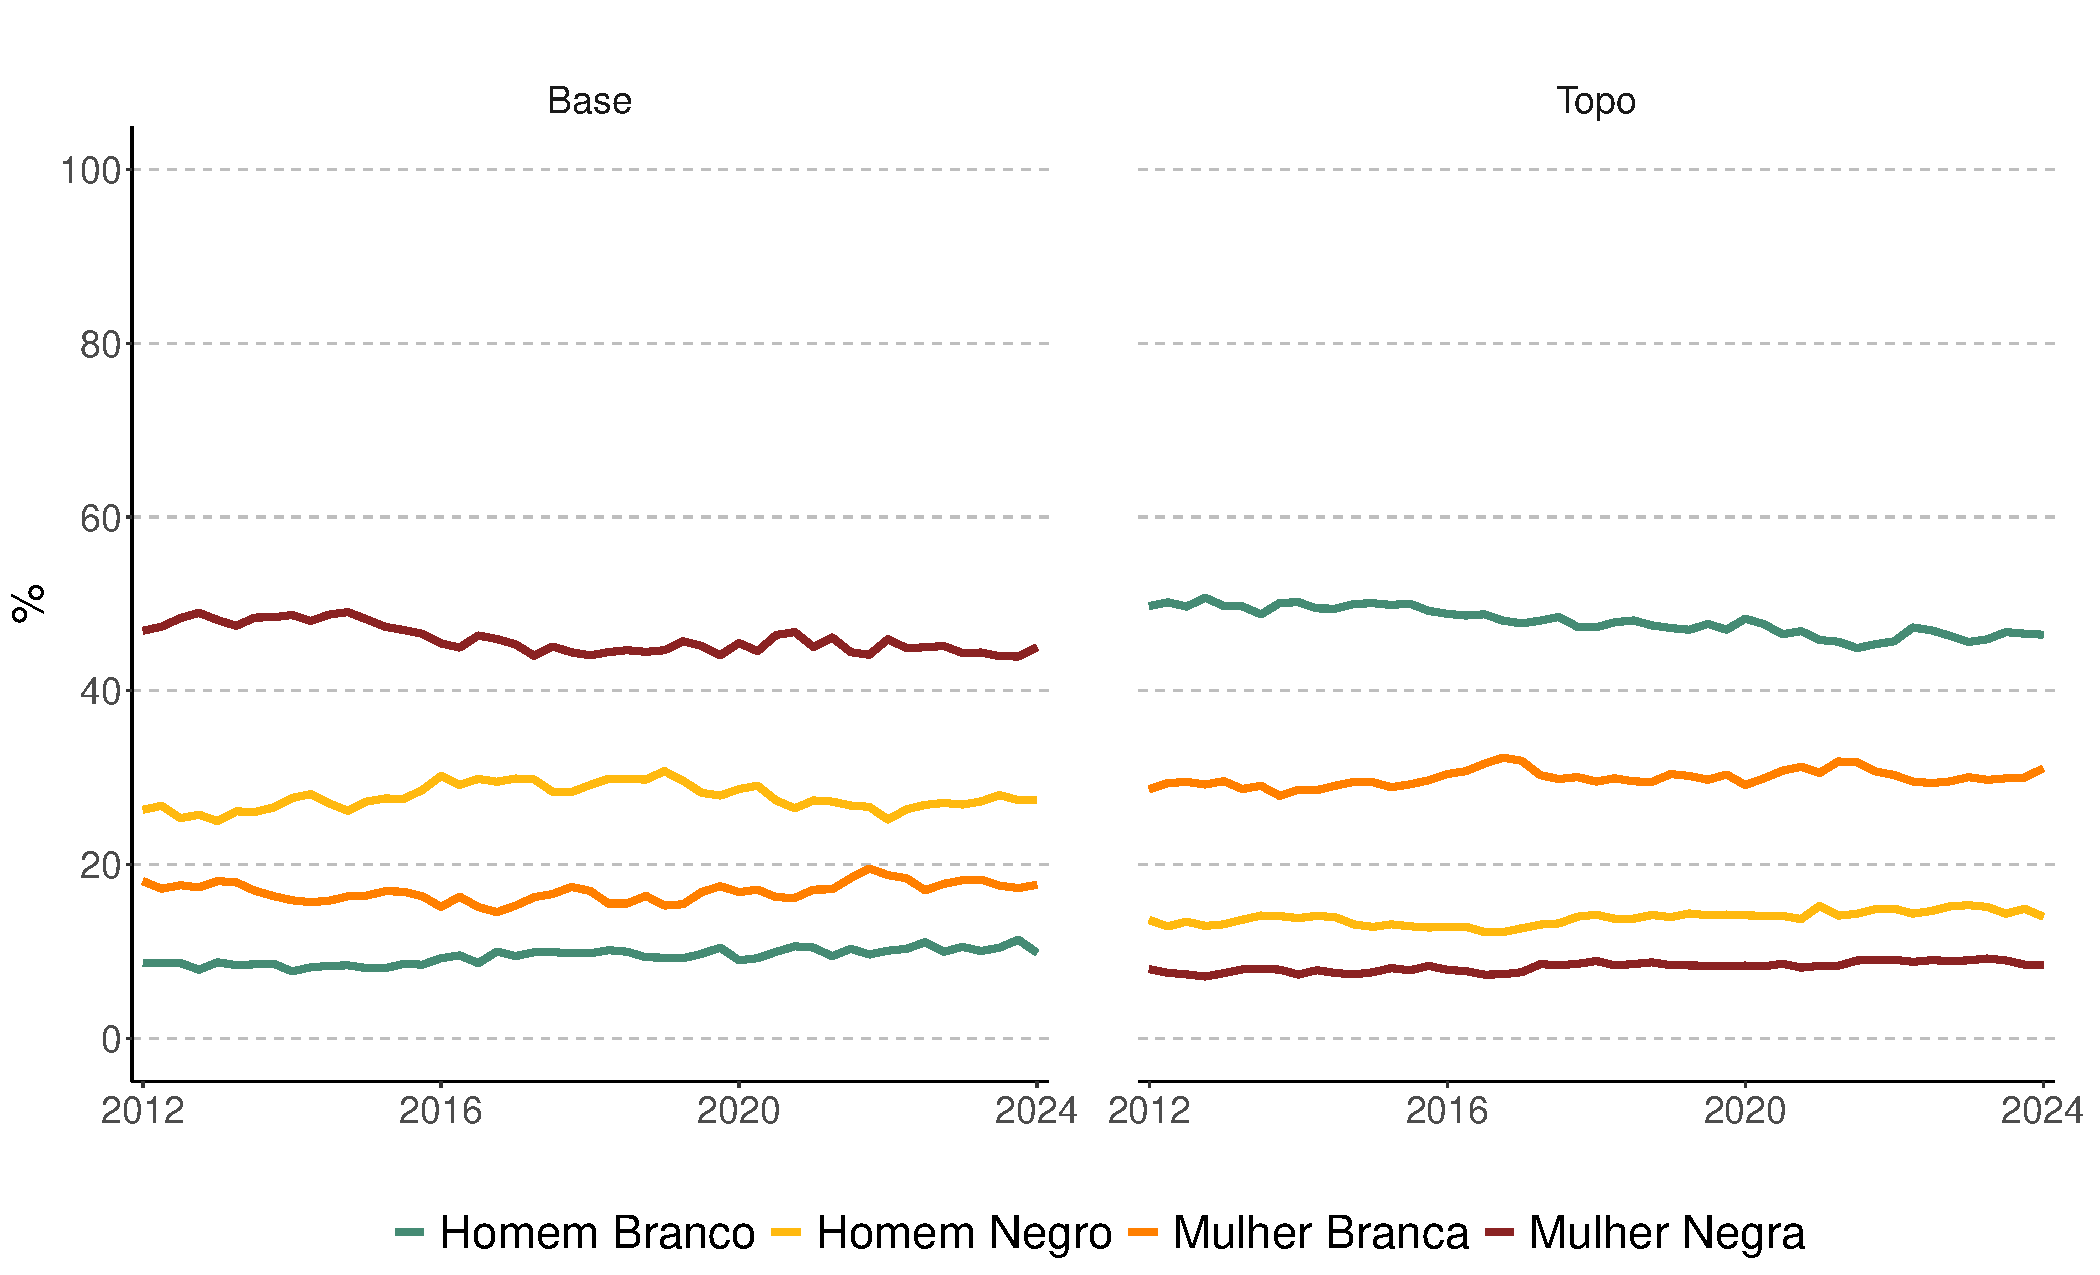
\includegraphics[width = 0.75\textwidth]{figures_output/base_topo_5_linha.pdf}
		\end{figure}
	\end{frame}
	
	\begin{frame}{Os dez por cento mais pobre e mais rico}
		\begin{figure}
			\centering
			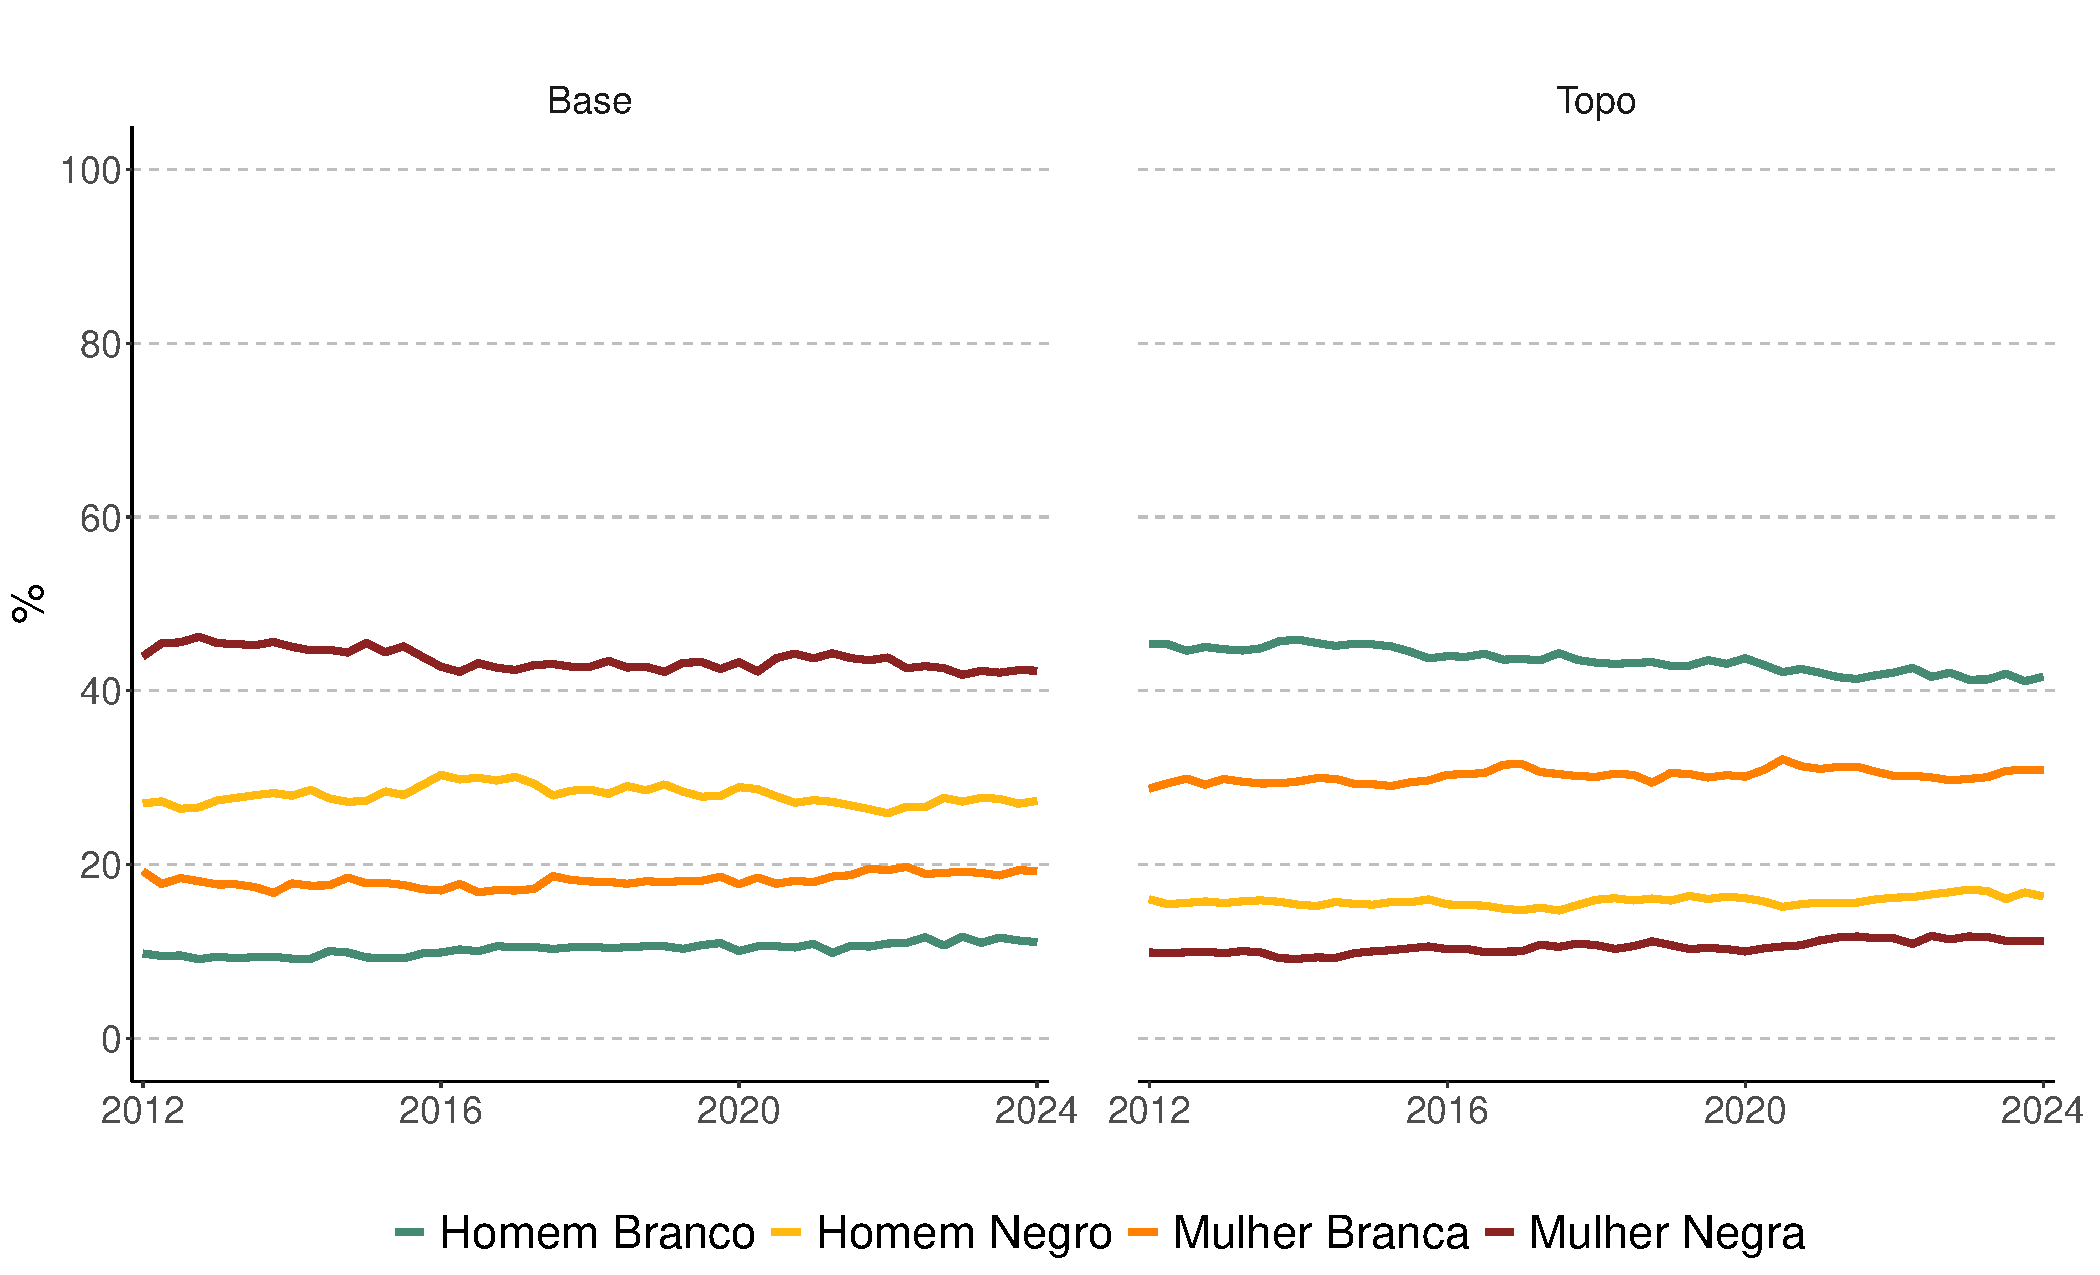
\includegraphics[width = 0.75\textwidth]{figures_output/base_topo_10_linha.pdf}
		\end{figure}
	\end{frame}
	
	\begin{frame}{Massa Salarial Recente}
		\begin{figure}
			\centering
			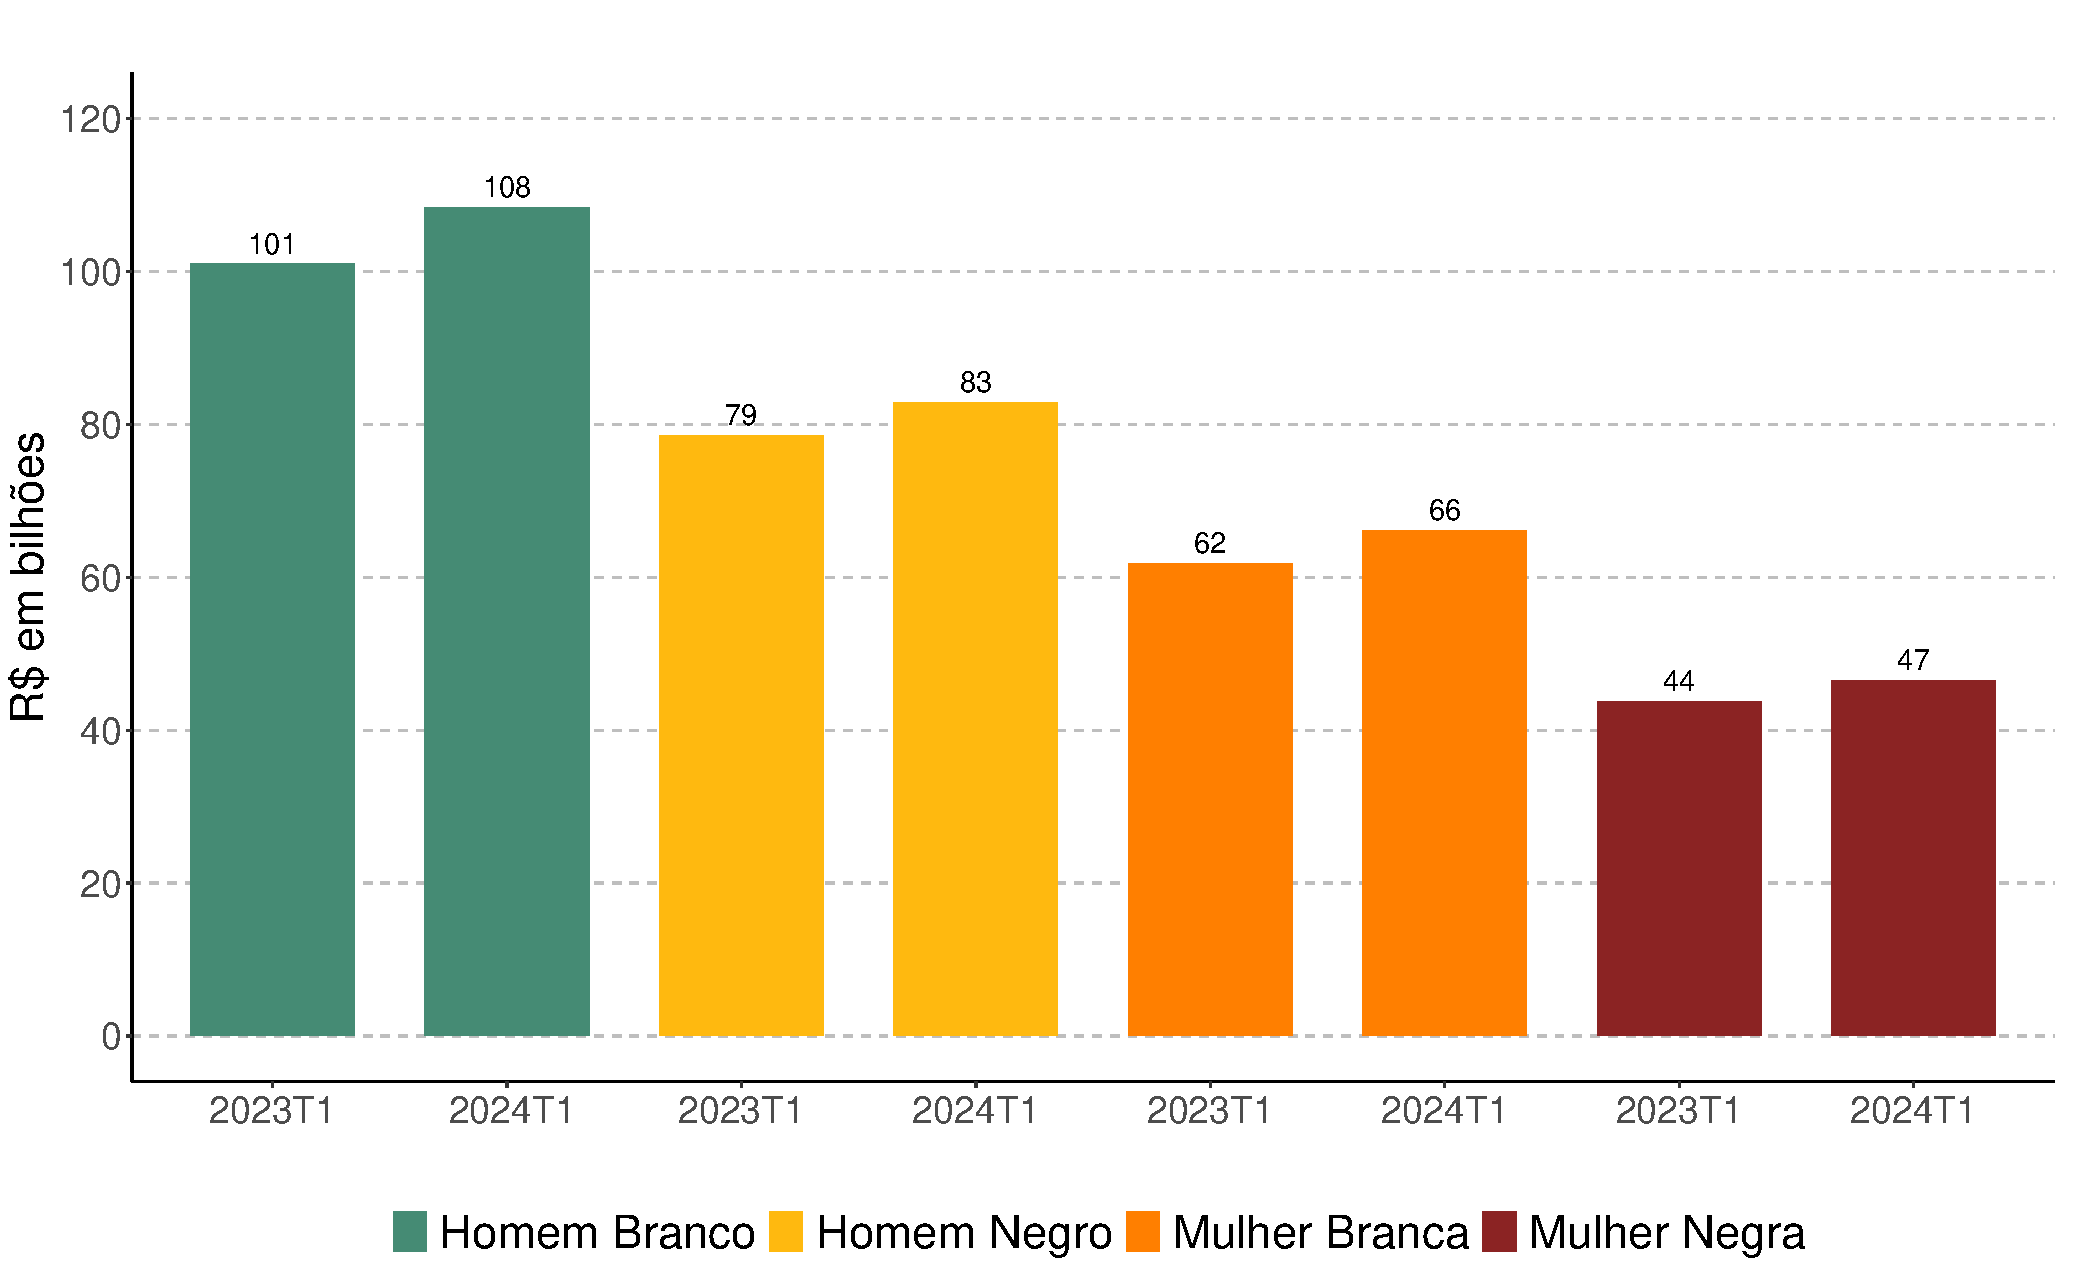
\includegraphics[width = 0.75\textwidth]{figures_output/massa_habitual.pdf}
		\end{figure}
	\end{frame}
	
	\begin{frame}{Massa Salarial Habitual}
		\begin{figure}
			\centering
			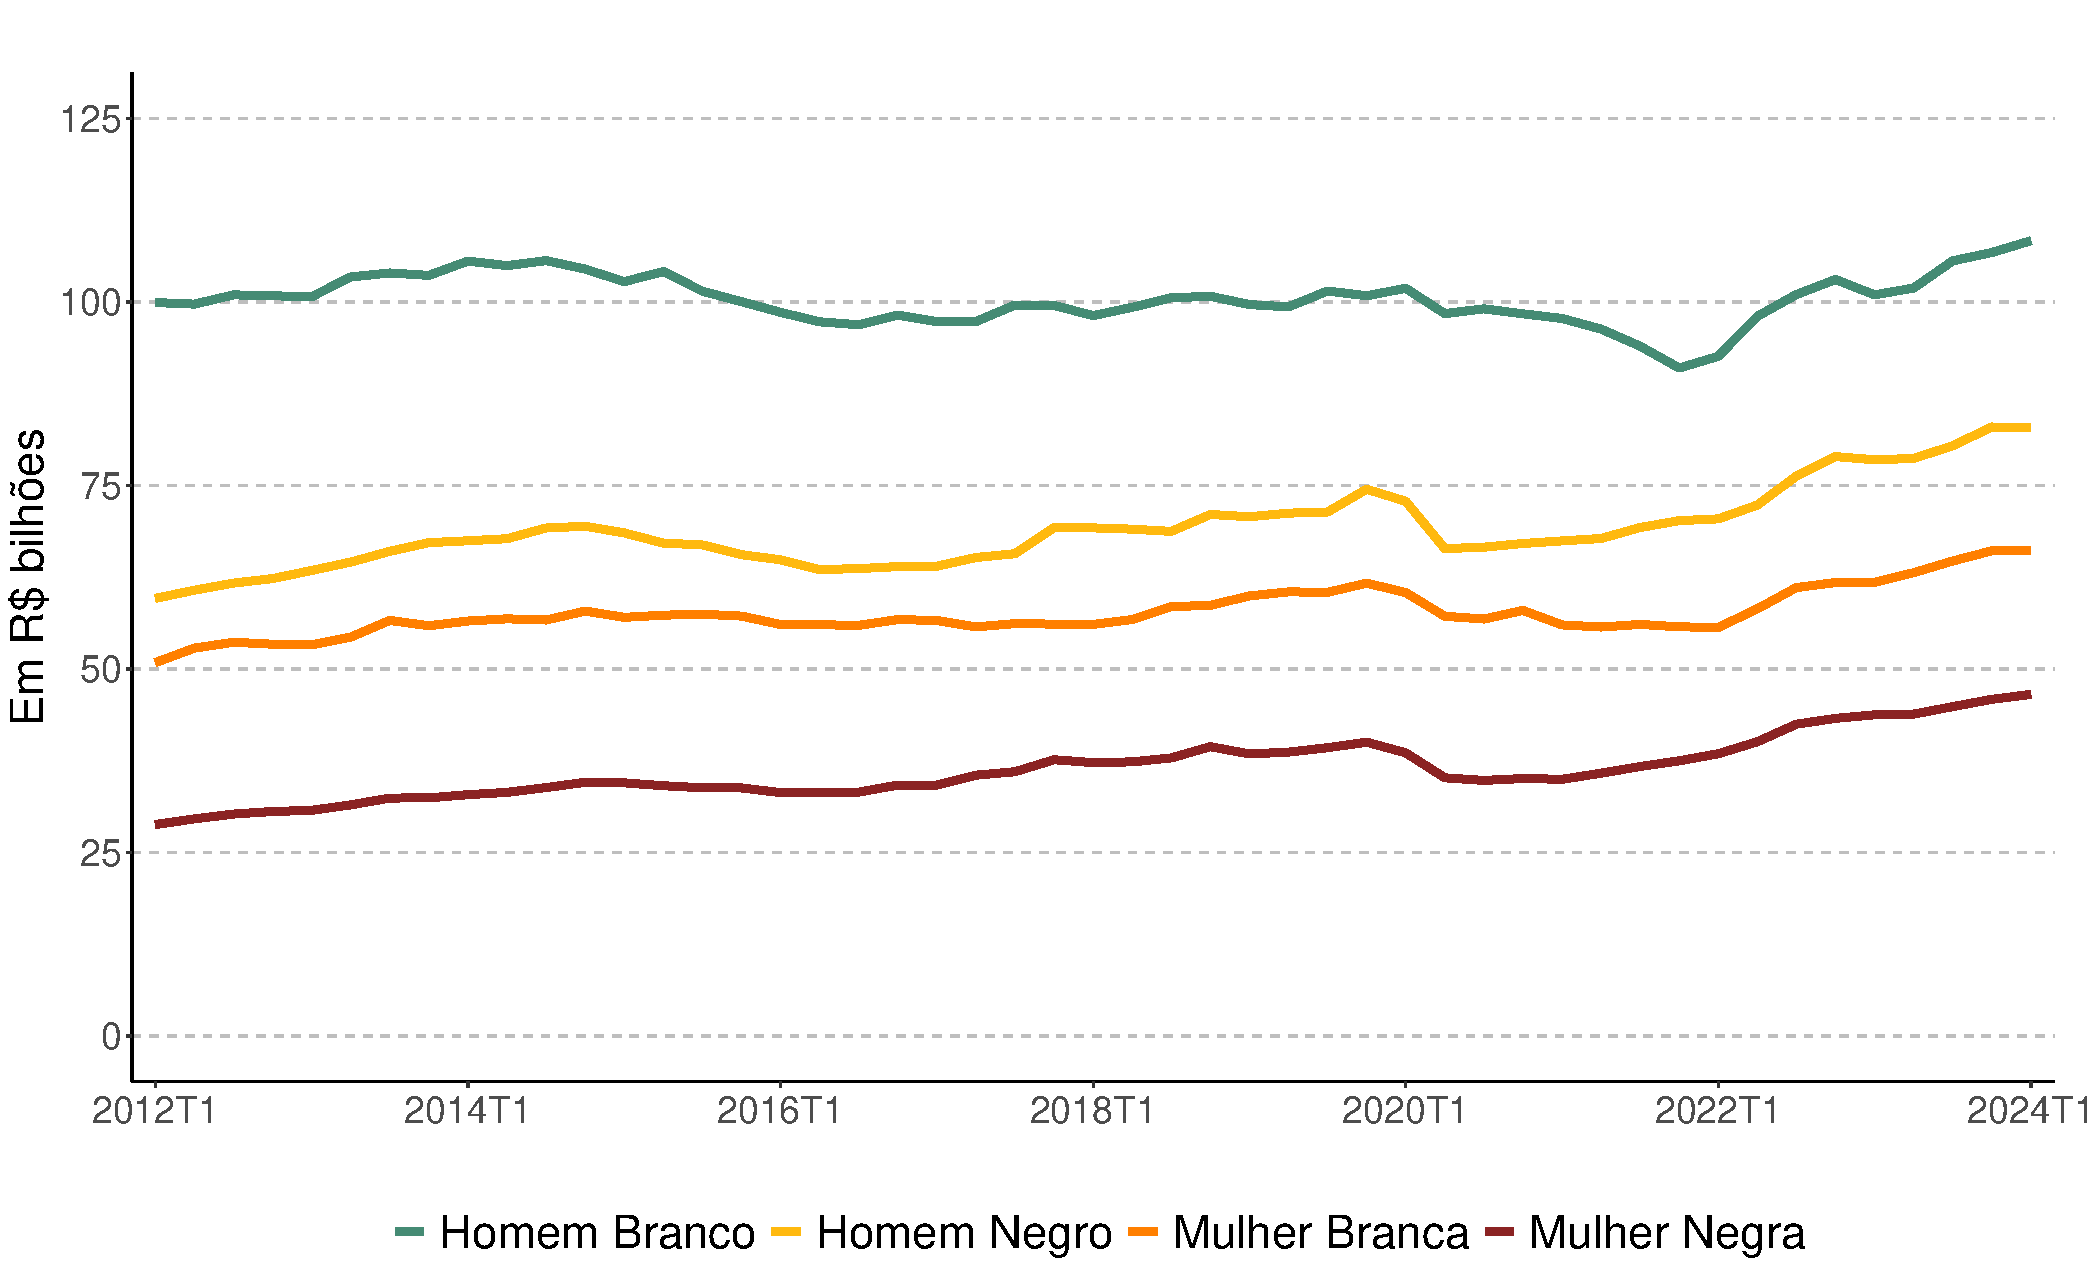
\includegraphics[width = 0.75\textwidth]{figures_output/massa_habitual_gen_raca.pdf}
		\end{figure}
	\end{frame}
	
	\begin{frame}{Desigualdade na Massa Salarial}
		\begin{figure}
			\centering
			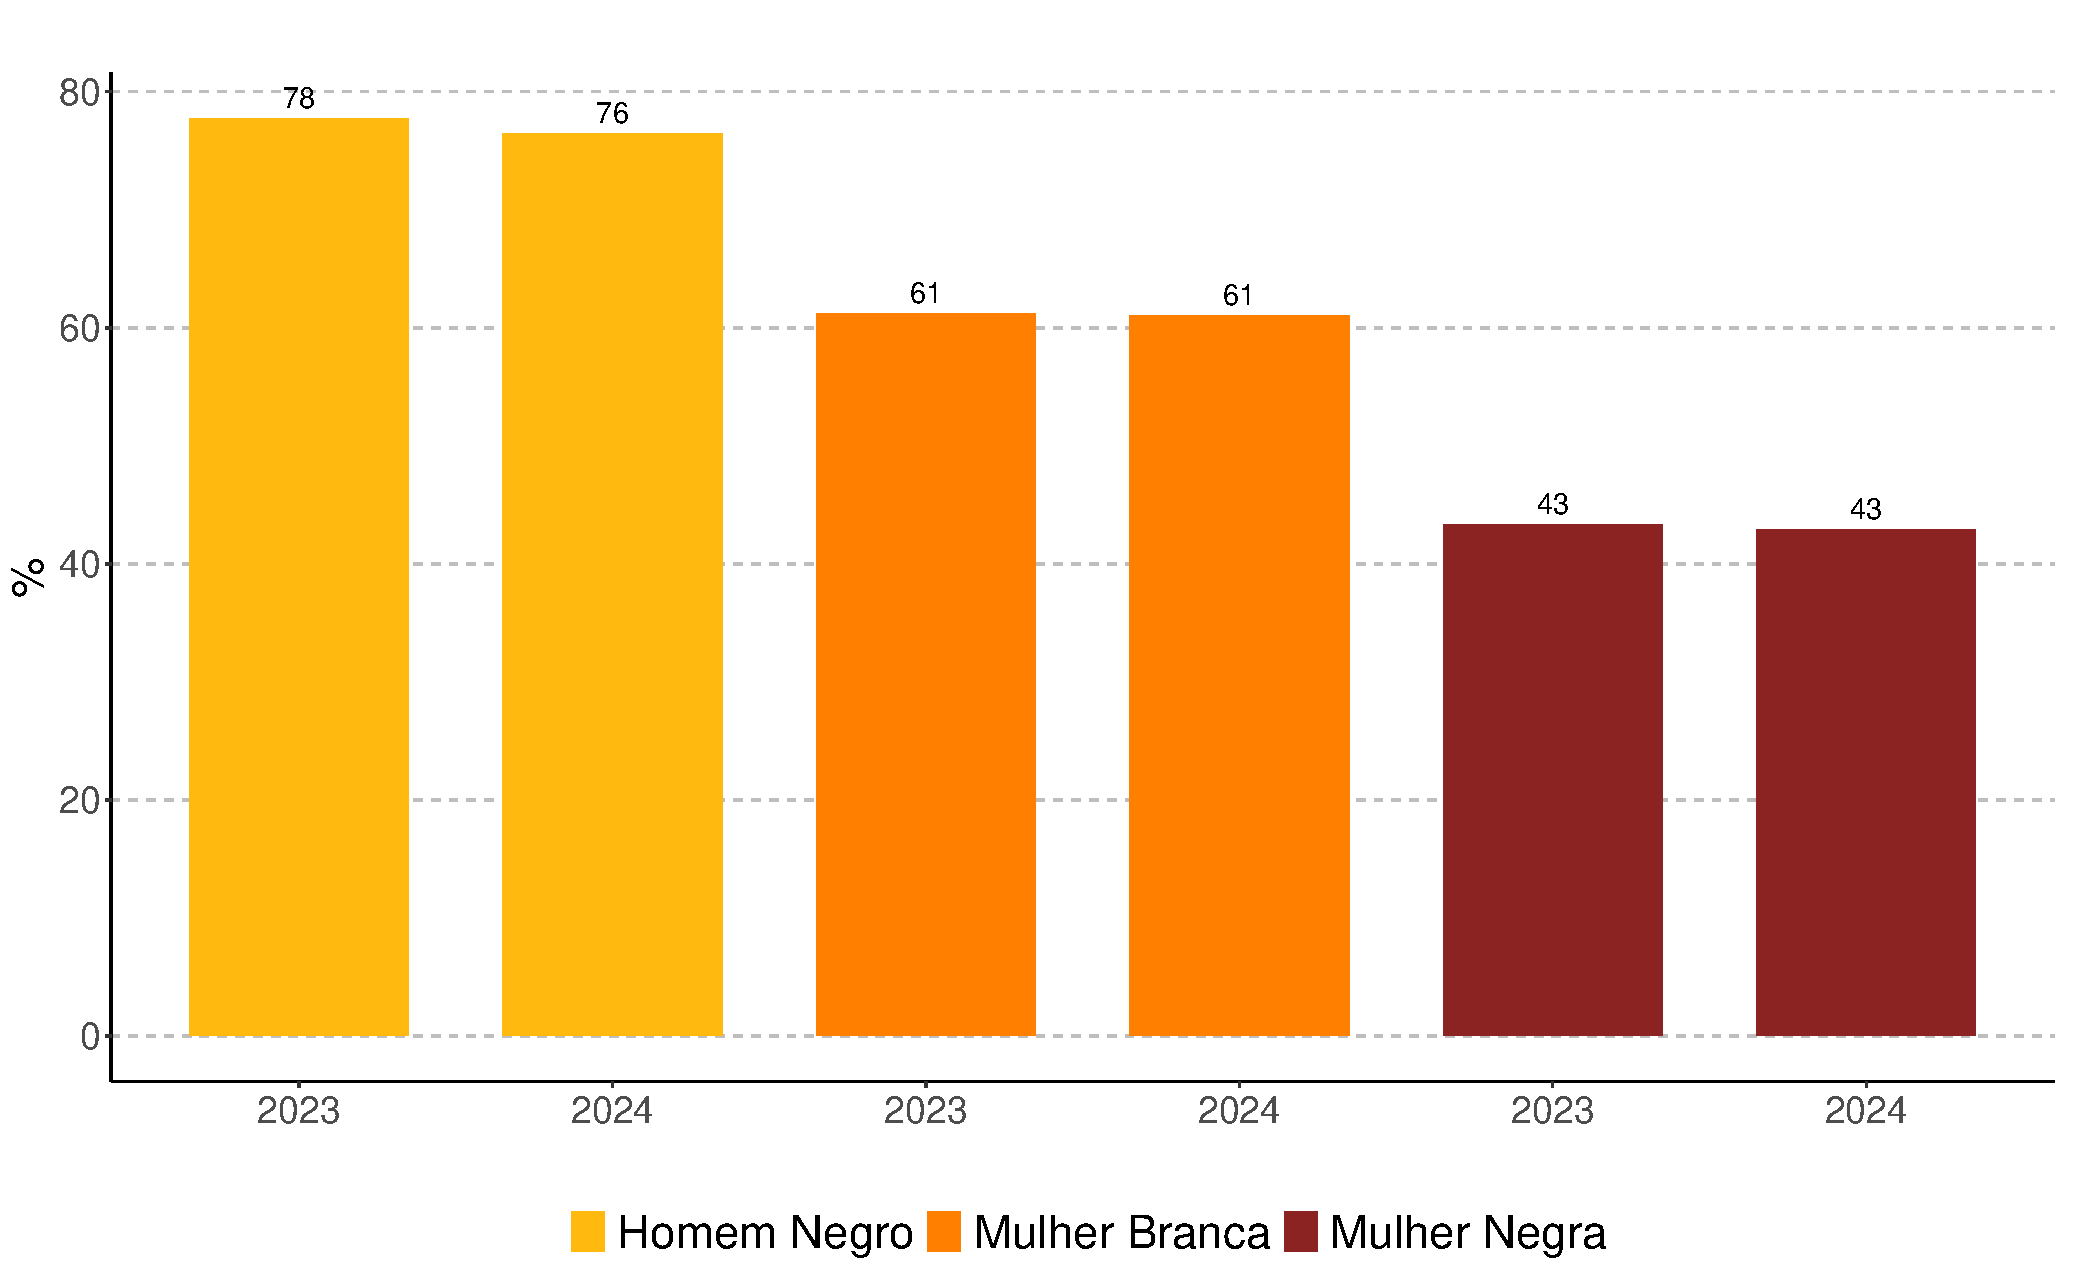
\includegraphics[width = 0.75\textwidth]{figures_output/frac_massa_habitual.pdf}
		\end{figure}
	\end{frame}		
	
	\section{Estimando a Massa Salarial Perdida para Desigualdade}
	\begin{frame}{A Massa Salarial}
	\begin{itemize}
		\item A massa salarial pode ser definida como o total de salários pagos a todos os trabalhadores em determinado período.
	\end{itemize}
	\begin{equation}
		M = \sum_{i =1}^{E} y_{i} = E \frac{\sum_{i =1}^{E} y_{i}}{E} = E \bar{Y}
	\end{equation}
	\begin{itemize}
		\item 	Onde: $E$ representa o total de trabalhadores, ou seja, $E = eP$; 
		\item	No qual, $e$ representa a proporção de pessoas que estão trabalhando e $P$ é o tamanho da população
		\item	$y_{i}$ representa o salário de cada trabalhador e $\bar{Y}$ representa a média salarial. 
	 \end{itemize}	
	\end{frame}	
	
	\begin{frame}{A Massa Salarial}
	\begin{itemize}
		\item Considere que há apenas dois grupos na economia: negros e brancos.
		\item Assim, a massa salarial é a soma da massa dos trabalhadores negros e com a massa dos trabalhadores brancos, logo:
	\end{itemize}
	\begin{equation}
	M =  P_{0}\bar{e}_{0} \bar{Y}_{0} + P_{1}\bar{e}_{1} \bar{Y}_{1} 
	\end{equation}
	\begin{itemize}
		\item 	Onde o subscrito 0 representa os indivíduos brancos e o 1 representa os negros. 
		\item	No qual, $e$ representa a proporção de pessoas que estão trabalhando e $P$ é o tamanho da população
		\item	$y_{i}$ representa o salário de cada trabalhador e $\bar{Y}$ representa a média salarial. 
	\end{itemize}	
\end{frame}	

	\begin{frame}{A Massa Salarial}
	\begin{itemize}
		\item 	Devido a diversos fatores negros e brancos tem gruas de empregabilidade e salário médio distintos. Considere, então a massa contrafactual, na qual tanto a renda média quanto a empregabilidade dos negros são iguais dos indivíduos brancos, temos então:
	\end{itemize}
	\begin{equation}
		M^{c} = P_{0}e_{0}\bar{Y}_{0} + P_{1}e_{0}\bar{Y}_{0}
	\end{equation}	
	\begin{itemize}
		\item 	De que forma podemos mensurar a massa salarial perdida devido à desigualdade racial no mercado de trabalho? Para isso, procedemos matematicamente da seguinte forma:
		\end{itemize}
	\begin{align}
	P_{0}e_{0}\bar{Y}_{0} + P_{1}e_{1}\bar{Y}_{1} \pm P_{1}e_{0}\bar{Y}_{0} &= P_{0}e_{0}\bar{Y}_{0} + P_{1}e_{1}\bar{Y}_{1} + P_{1}e_{0}\bar{Y}_{0} - P_{1}e_{0}\bar{Y}_{0} \\
	&= (P_{0} +  P_{1})e_{0}\bar{Y}_{0} + P_{1}(e_{1}\bar{Y}_{1} - e_{0}\bar{Y}_{0})
	\end{align}
	\end{frame}	

	\begin{frame}{A Massa Salarial}
	\begin{itemize}
		\item A equação (5) não permite decompor a perda da massa salarial em termos salariais e em termos de empregabilidade.
		\item 	Para isso, torna-se necessária a seguinte manipulação algébrica: 
	\end{itemize}
		\begin{equation}
		M^{c} + P_{1}(\bar{e}_{1}\bar{Y}_{1} - \bar{e}_{0}\bar{Y}_{0} + \bar{e}_{1}\bar{Y}_{0} - \bar{e}_{1}\bar{Y}_{0}) = M^{c} + P_{1}(\bar{e}_{1}\bar{Y}_{1} - \bar{e}_{1}\bar{Y}_{0} + \bar{e}_{1}\bar{Y}_{0} - \bar{e}\bar{Y}_{0})
	\end{equation}
	
	\begin{equation}
		M^{c} + P_{1}[e_{1}(\bar{Y}_{1} - \bar{Y}_{0}) + \bar{Y}_{0}(\bar{e}_{1} - \bar{e} )] =  M^{c} + P_{1}[e_{1}\Delta \bar{Y}_{(1,0)} + \bar{Y}_{0}\Delta \bar{e}_{(1,0)}]
	\end{equation}
	\begin{itemize}
		\item Onde: $e_{1}\Delta \bar{Y}_{(1,0)}$ é a penalidade salarial e,
		\item 	$\bar{Y}_{0}\Delta \bar{e}_{(1,0)}$ é a penalidade na empregabilidade.
		\end{itemize}
	\end{frame}	
		
	\begin{frame}{A Equação Salarial}
		\begin{itemize}
			\item A equação salarial pode ser estimada do seguinte modo:
		\end{itemize}
			\begin{equation}
			{Y}_{i} = \alpha + X_{i}\beta +  \gamma_{i} + \epsilon_{i}
		\end{equation}	
		\begin{itemize}
			\item Onde $X_{i}$ representa o conjunto de características observadas dos trabalhadores $i$ como escolaridade, experiência, vínculo empregatício, setor da economia. E $\gamma$ indica se o trabalhador é negro.
			\item E o salário médio pode ser estimado da seguinte forma:
		\end{itemize}
			\begin{equation}
			\bar{Y} =  \frac{\sum_{i=1}^{E}{Y}_{i}}{E}
		\end{equation}	
		\end{frame}
		
		
	\begin{frame}{A Equação Salarial}
	\begin{itemize}
		\item Considere agora que a discriminação racial foi abolida. Nesse contrafactual, o salário estimado dos trabalhadores negros seria:
	\end{itemize}
	\begin{equation}
		{Y}_{c} = \alpha + X_{i}\beta + \epsilon_{i}
	\end{equation}	
	\begin{itemize}
	\item A diferença entre o salário médio dos negros no cenário com discriminação em relação ao resultado médio contrafactual mensura a perda salarial média devido à discriminação no mercado de trabalho. Ou seja, 
	\end{itemize}
	\begin{equation}
	\bar{Y}_{1}  - \bar{Y}_{c}  =  \gamma
	\end{equation}	
	\begin{itemize}
	\item Enquanto a diferença salarial entre negros e brancos é mensurada como a diferença das variáveis observadas, que é chamada de efeito composição, expresso por $\bar{Y}_{c} - \bar{Y}_{0}$.
	\item Assim, a penalidade salarial é a soma dos efeitos composição e discriminação = $(\bar{Y}_{c} - \bar{Y}_{0}) + \gamma$.
	\end{itemize}
	\end{frame}
	
	\begin{frame}{A Equação da Empregabilidade}
		\begin{itemize}
			\item Até agora vimos o aspecto salarial no mercado de trabalho. No entanto, compreender a dinâmica da discriminação racial no mercado de trabalho envolve em entender como isso afeta a empregabilidade.
			\item Para isso, temos a seguinte função que mensura a probabilidade do indivíduo estar empregado
		\end{itemize}
		\begin{equation}
			e_{i} = \theta + Z_{i}\phi + \delta_{i} + \mu_{i}
		\end{equation}
		\begin{itemize}
			\item Temos que a probabilidade média do individuo estar empregado:
		\end{itemize}
		\begin{equation}
			\bar{e}_{0} = \frac{\sum_{i=1}^{P}{e}_{i}}{P}
		\end{equation}
	\end{frame}
	
	\begin{frame}{A Equação da Empregabilidade}
		\begin{itemize}
			\item Tal como na equação salarial, iremos considerar um cenário contrafactual no qual a discriminação foi extinta. Nesse caso, temos que a probabilidade de uma pessoa negra estar empregada é estimada da seguinte forma:
		\end{itemize}
		\begin{equation}
				\bar{e_{c}} = \theta + Z_{i}\phi + \mu_{i}
		\end{equation}
		\begin{itemize}
			\item A probabilidade média do negro estar empregado baseado na diferença do resultado em um mercado de trabalho com discriminação em relação a um mercado sem discriminação é o nosso $\delta$.
			\item $ \bar{e}_{1} - \bar{e}_{c}= \delta$
			\item Ainda no cenário contrafactual, temos que, $\bar{e_{c}} \neq \bar{e_{0}}$ e o resultado dessa diferença é o efeito composição.
		\end{itemize}
	\end{frame}
	
		\section{Resultados}
		\begin{frame}{ Resultados da Perda da Massa Salarial}
		\begin{figure}
			\centering
			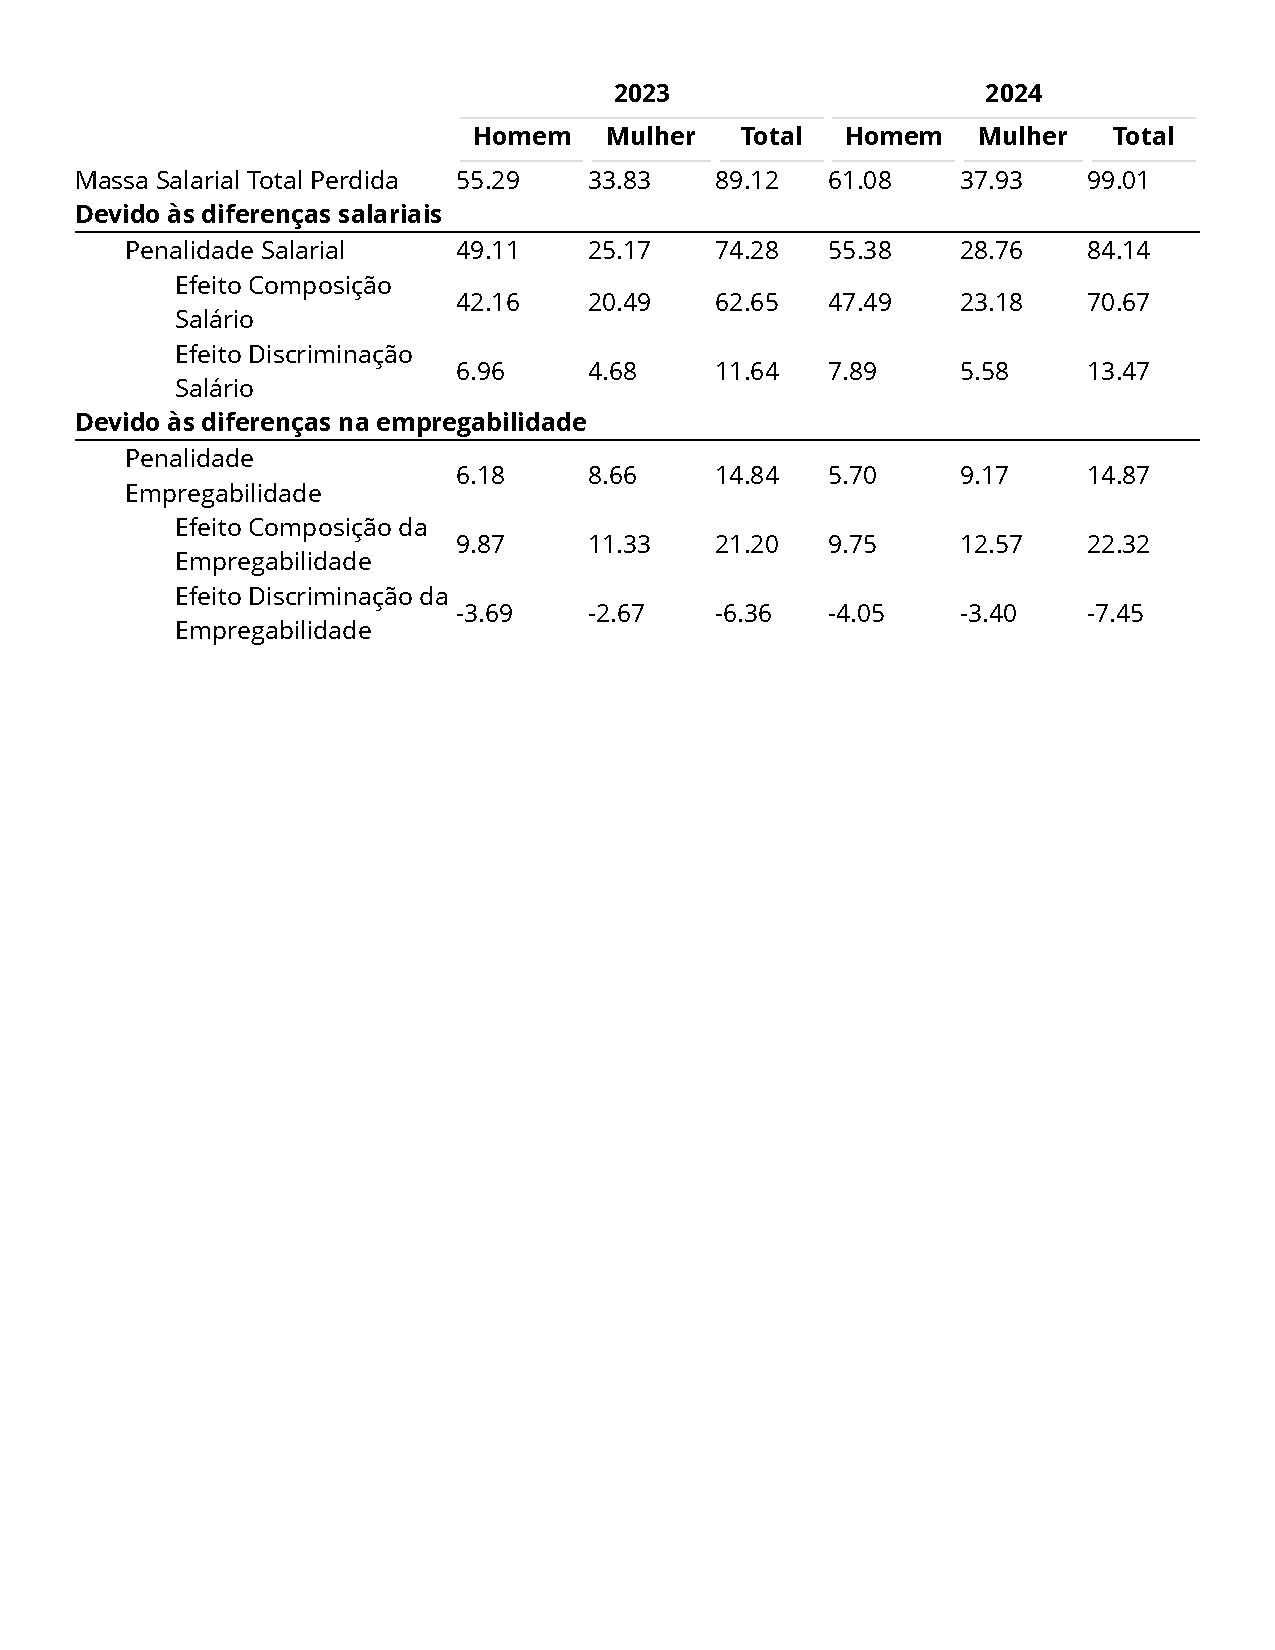
\includegraphics[width = 0.75\textwidth]{tables_output/table_massa.pdf}
		\end{figure}
		\end{frame}		
		
		\begin{frame}{ Perda Salarial Média e Probabilidade em estar Empregado}
		\begin{figure}
			\centering
			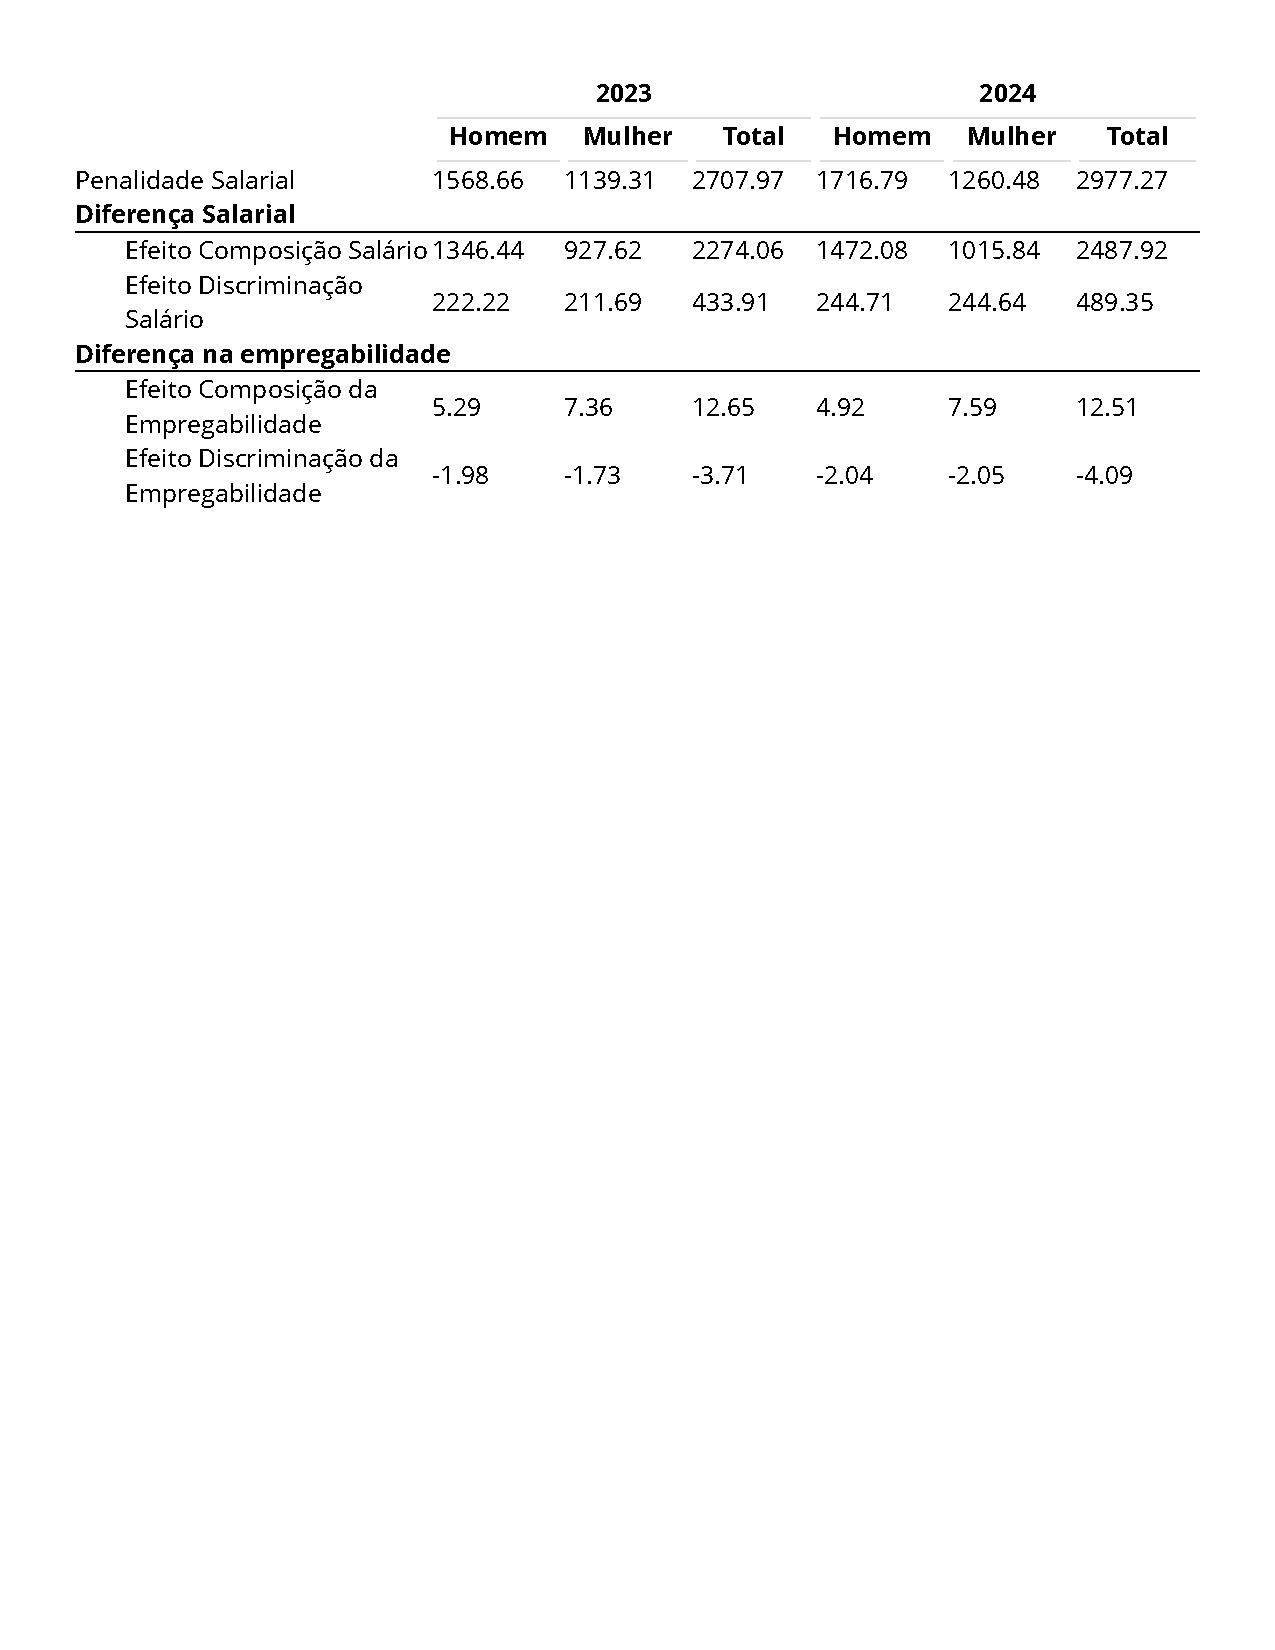
\includegraphics[width = 0.75\textwidth]{tables_output/table_individual.pdf}
		\end{figure}
		\end{frame}	
		
	\begin{frame}{A Massa Salarial Perdida - Homens Negros}
	\begin{figure}
		\centering
			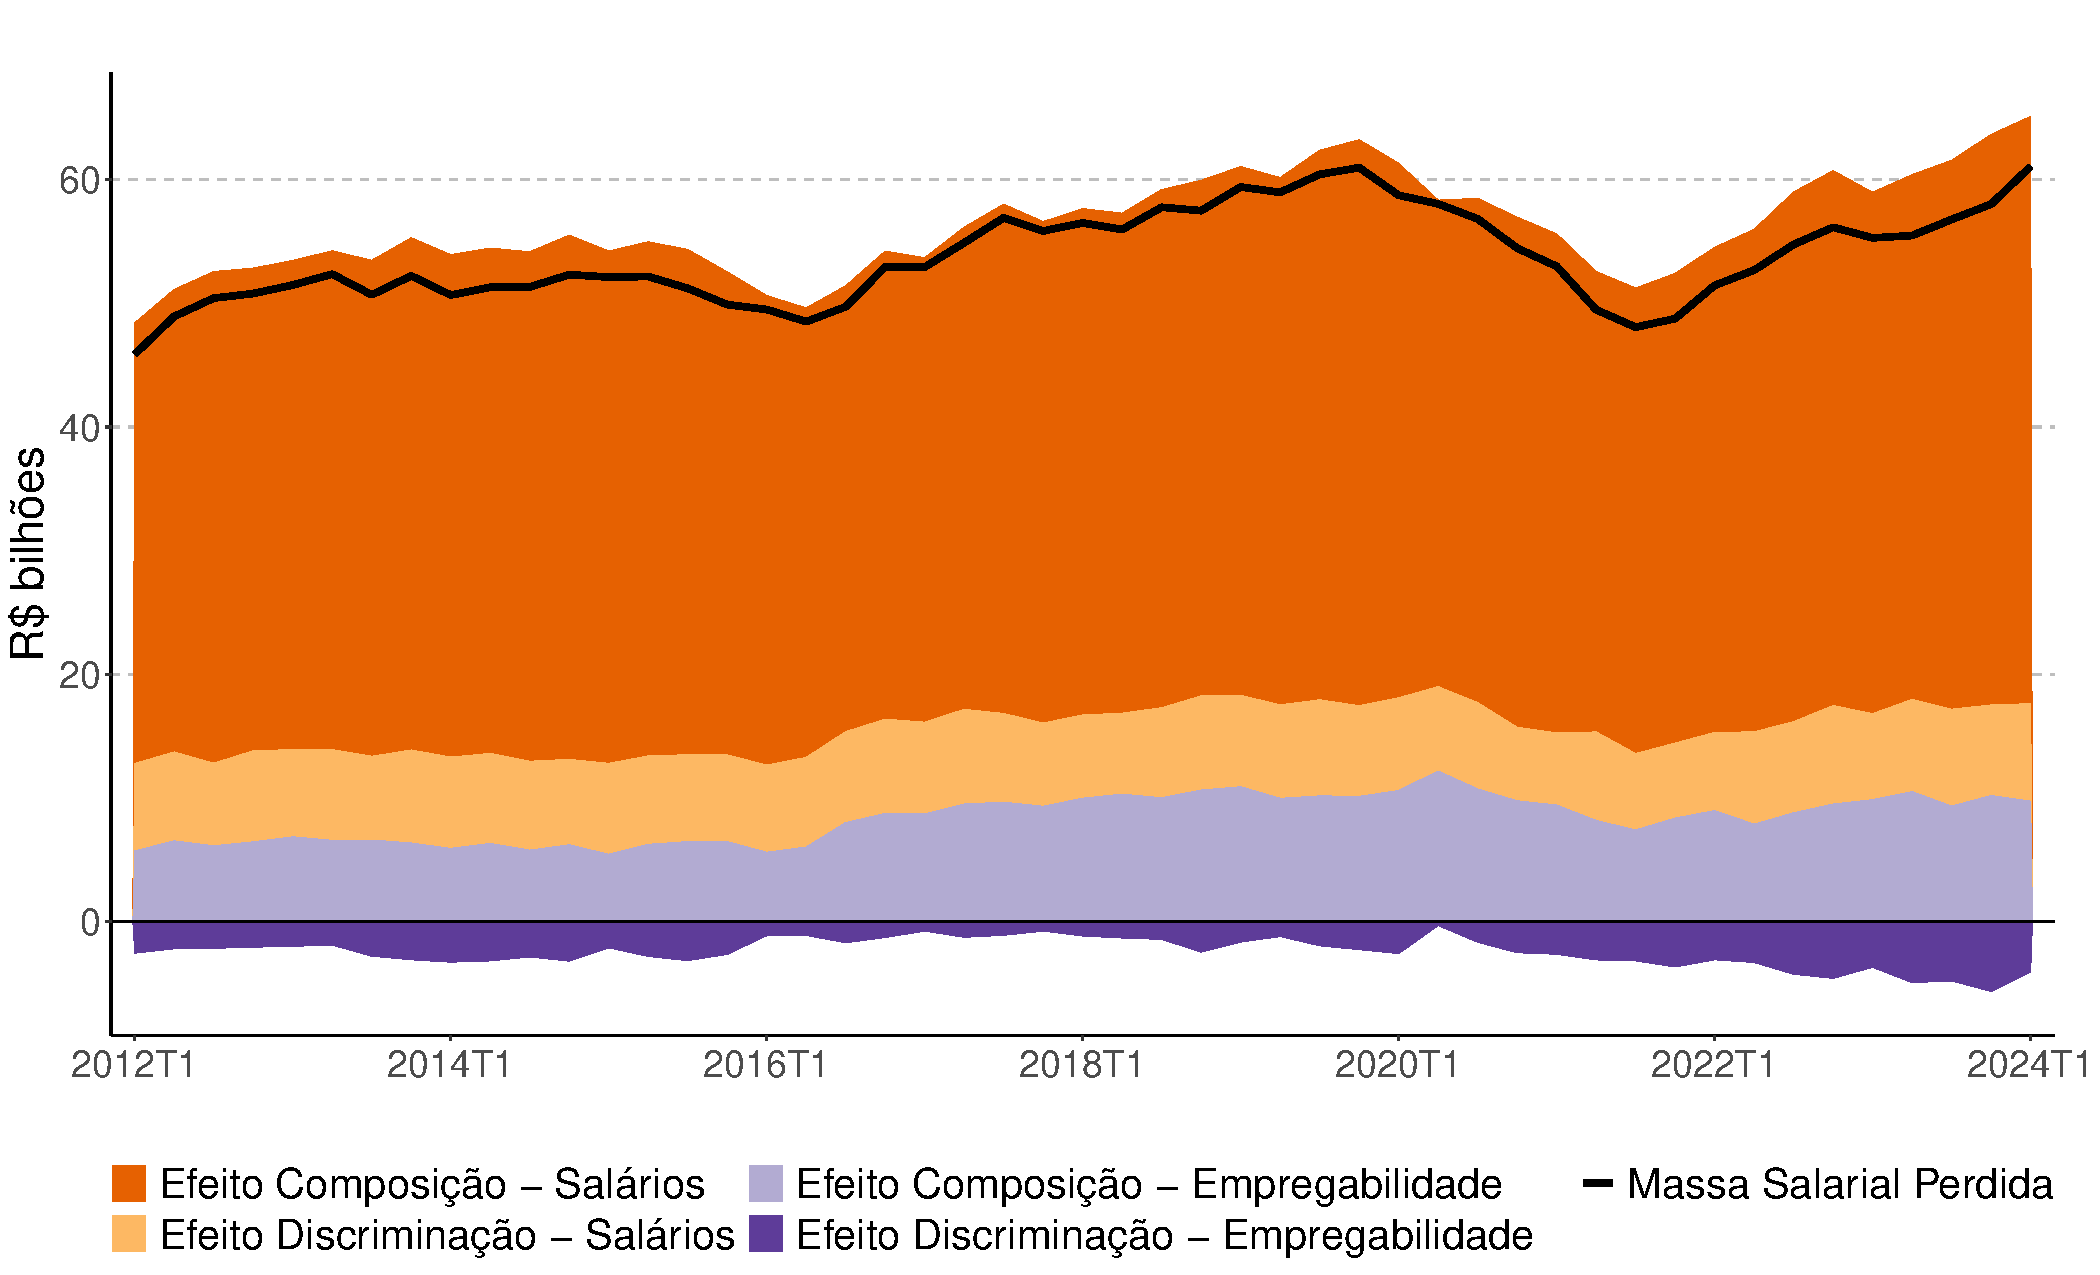
\includegraphics[width = 0.75\textwidth]{figures_output/homem_negro_massa_perdida_gph.pdf}
	\end{figure}
	\end{frame}	
	
	\begin{frame}{A Massa Salarial Perdida - Mulheres Negras}
	\begin{figure}
		\centering
		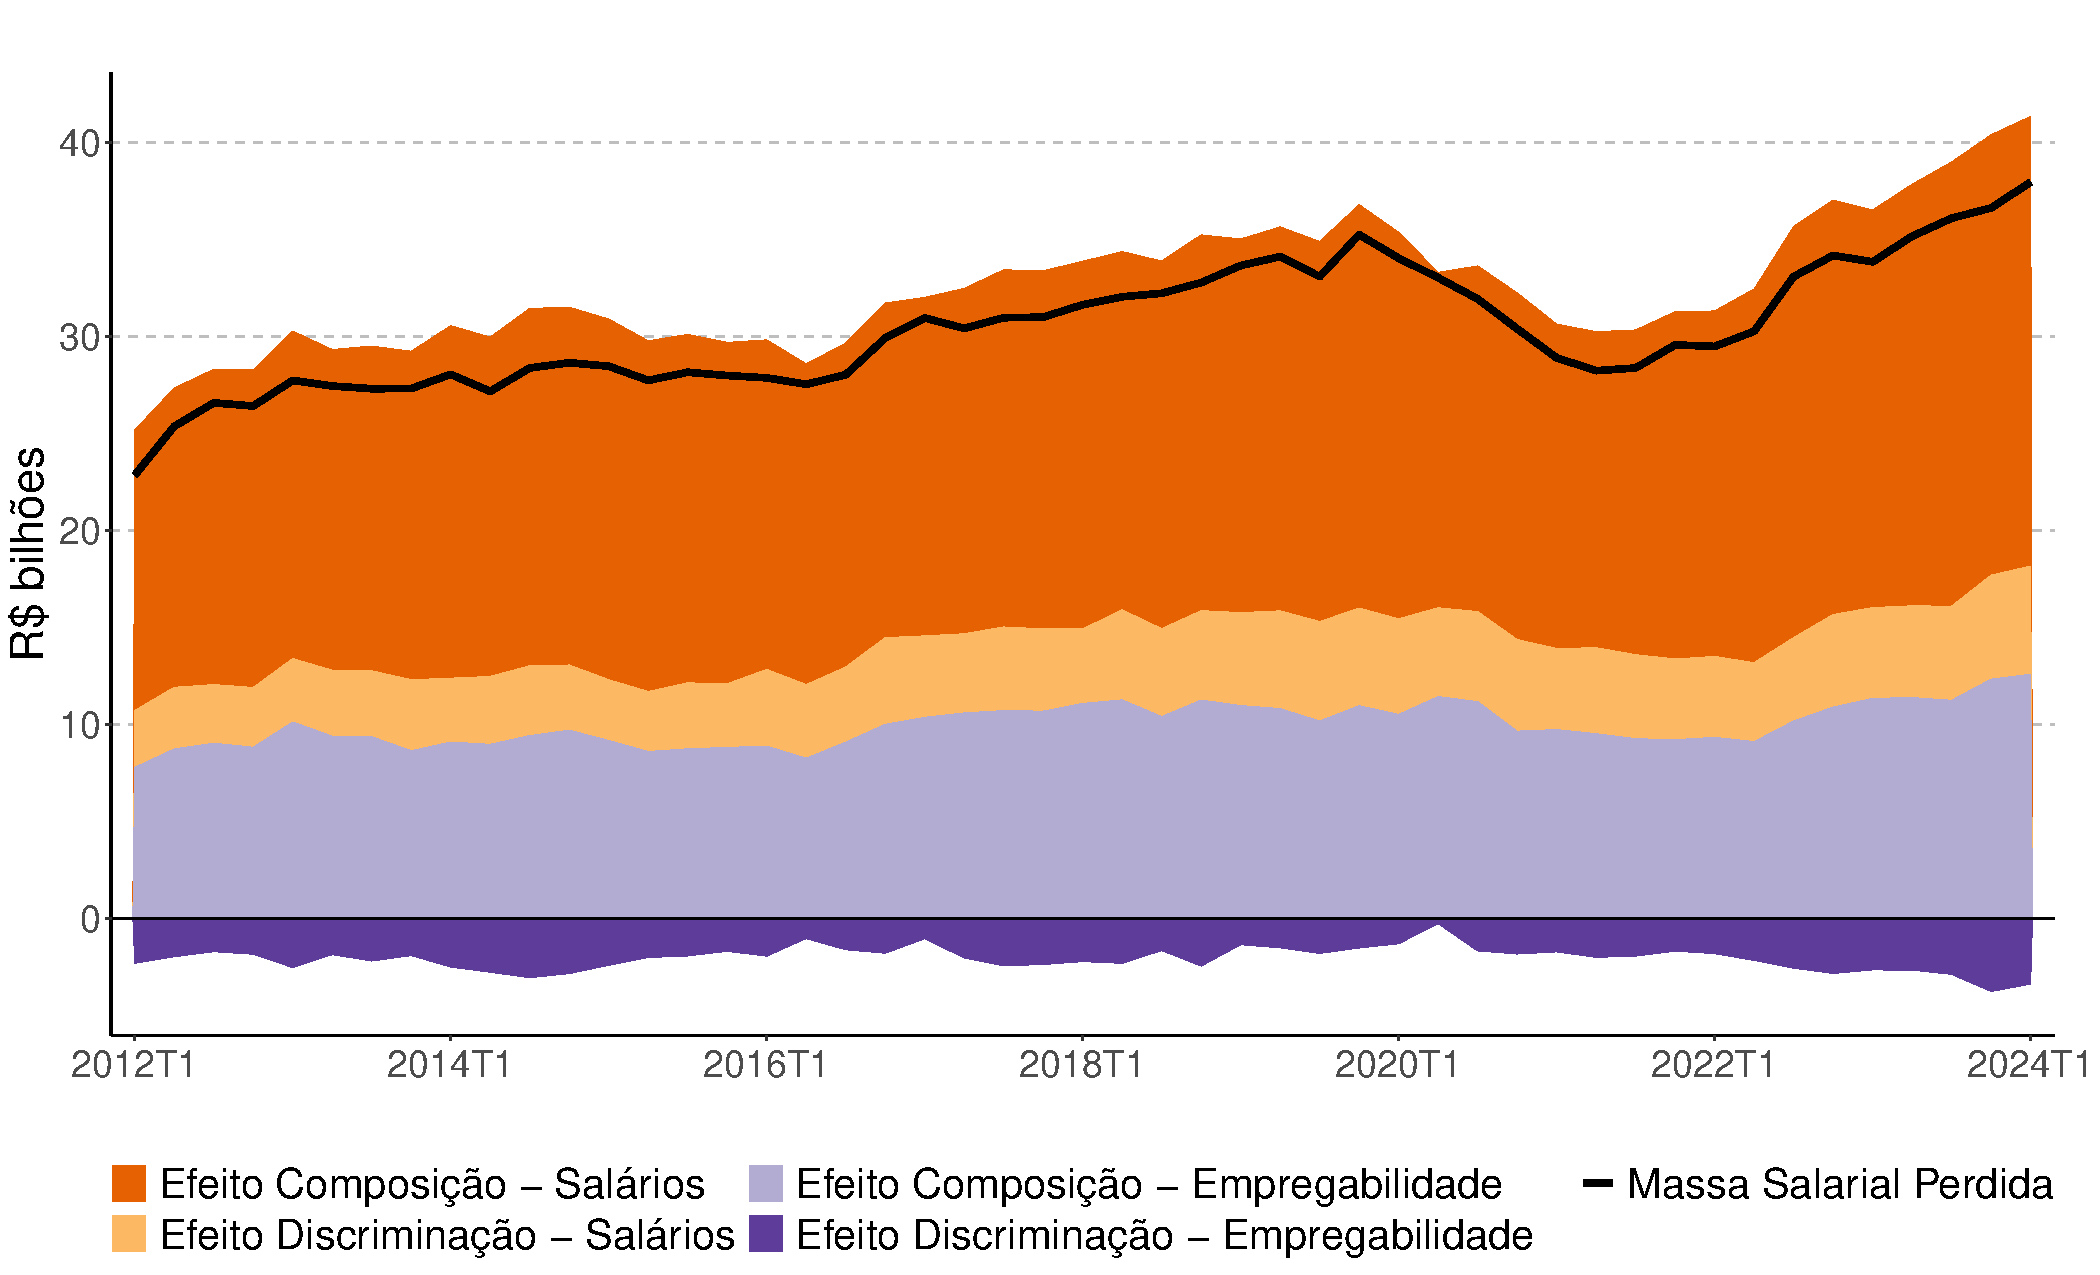
\includegraphics[width = 0.75\textwidth]{figures_output/mulher_negra_massa_perdida_gph.pdf}
	\end{figure}
	\end{frame}		
	
	\begin{frame}{A Massa Salarial Perdida dos Trabalhadores Negros}
	\begin{figure}
		\centering
		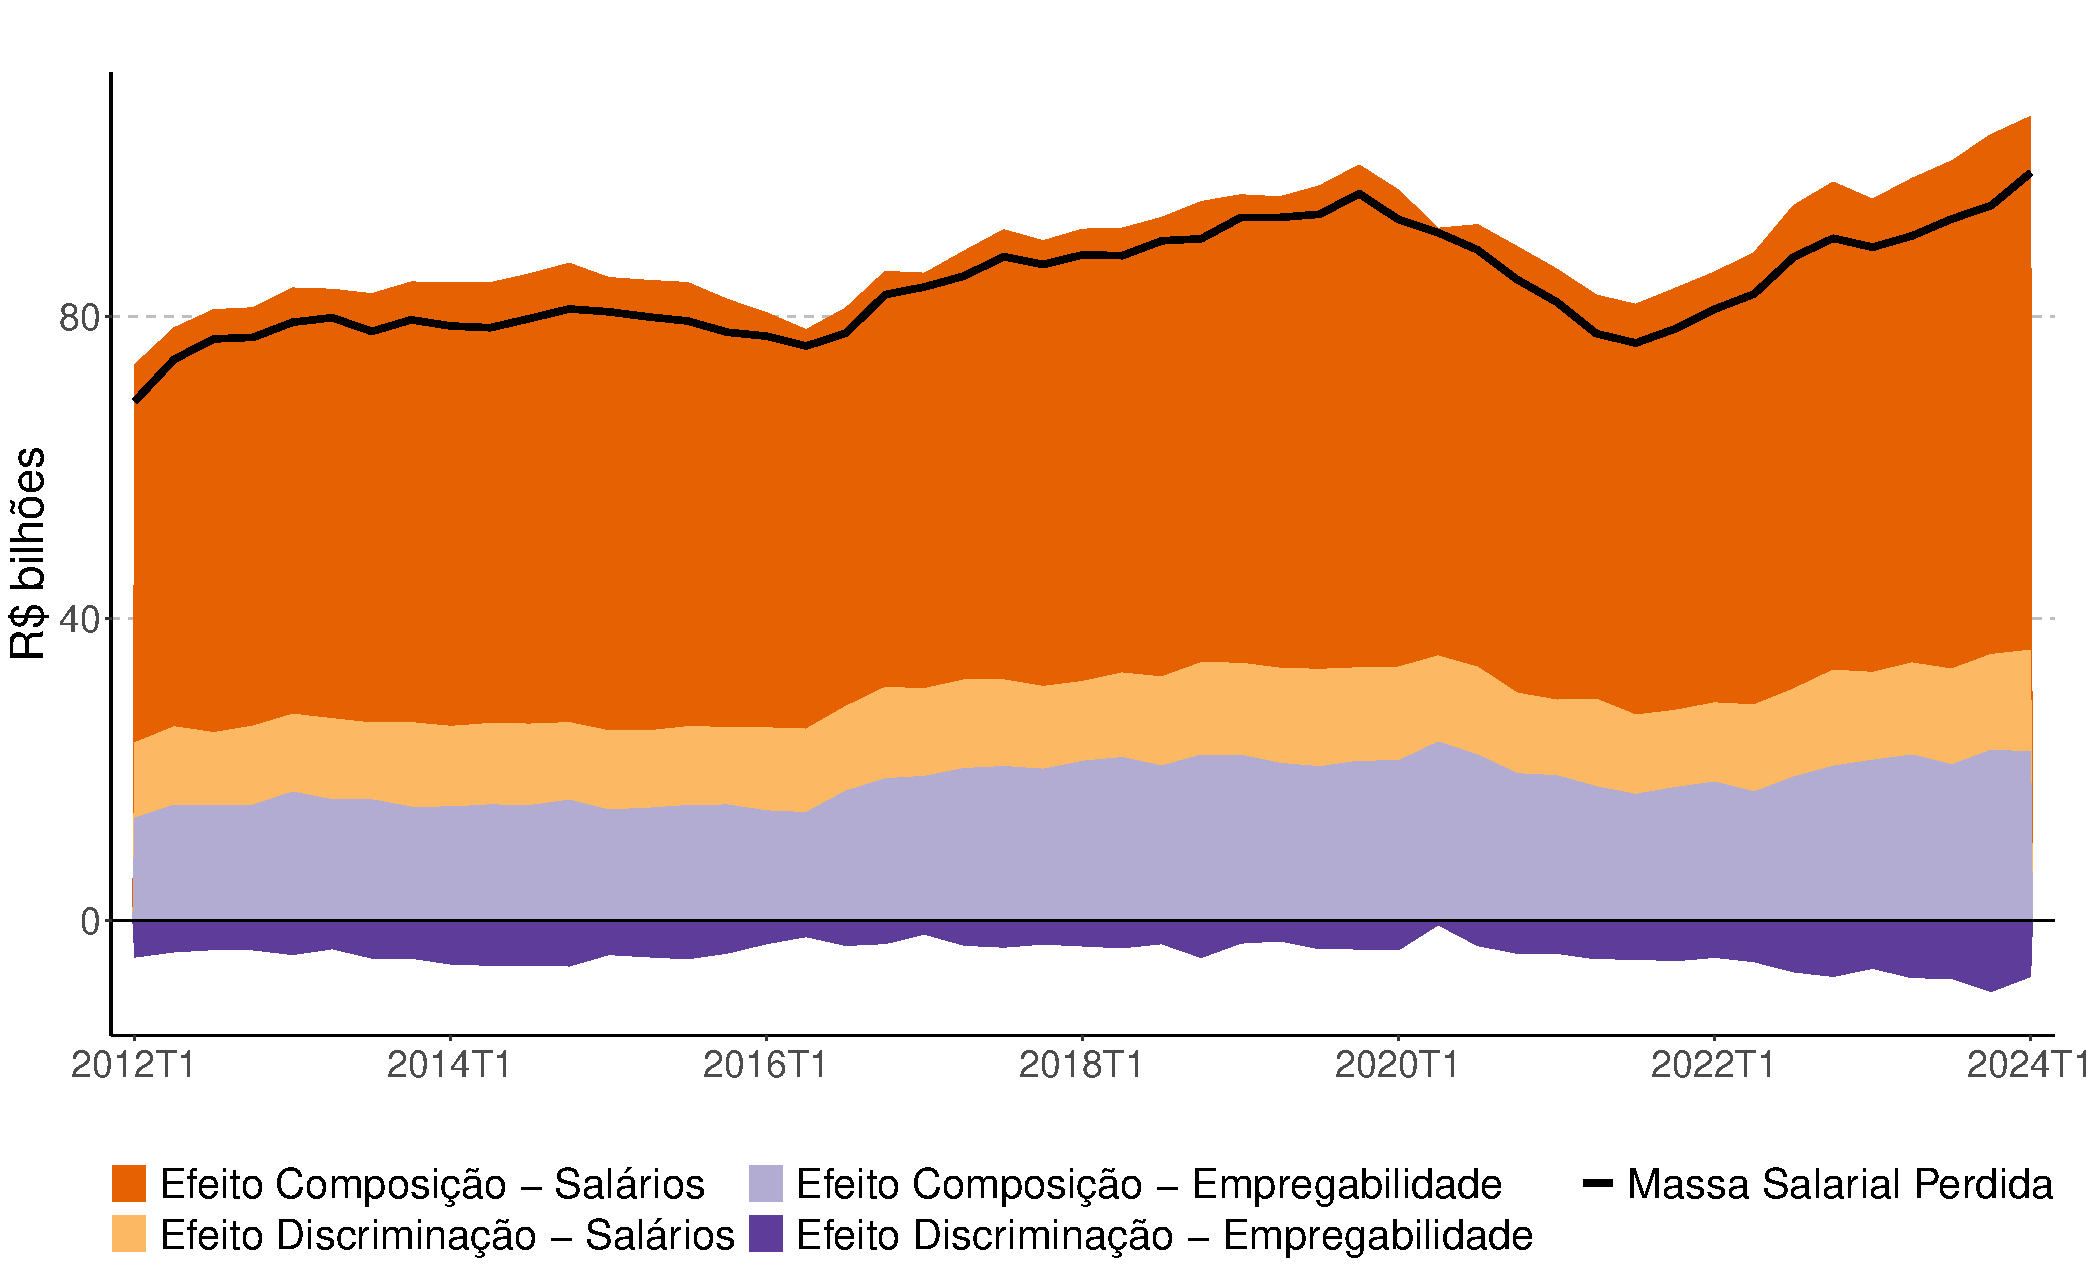
\includegraphics[width = 0.75\textwidth]{figures_output/massa_perdida_gph.pdf}
	\end{figure}
	\end{frame}		
		
\end{document}